\documentclass[conference]{IEEEtran}

\usepackage[utf8]{inputenc}
\usepackage[T1]{fontenc}
\usepackage{cite}
\usepackage{amsmath,amssymb,amsfonts}
\usepackage{graphicx}
\usepackage[caption=false,font=footnotesize]{subfig}
\usepackage{booktabs}
\usepackage{array}
\usepackage{multirow}
\usepackage{xcolor}
\usepackage{tikz}
\usepackage{pgfplots}
\usepackage{url}
\usepackage[hidelinks,unicode]{hyperref}

\pgfplotsset{compat=1.16}
\usetikzlibrary{arrows.meta,positioning,fit,shapes.geometric,calc}

\renewcommand{\refname}{Referencias}

\definecolor{aireTeal}{HTML}{0F766E}
\definecolor{aireBlue}{HTML}{1D4ED8}
\definecolor{aireAmber}{HTML}{D97706}
\definecolor{aireRed}{HTML}{DC2626}
\definecolor{aireGreen}{HTML}{22C55E}
\definecolor{aireGray}{HTML}{9CA3AF}
\definecolor{aireSlate}{HTML}{334155}

\begin{document}

\title{Aire-Trujillo: Plataforma IoT Solar LTE-M/GNSS Multiparamétrica, Firmware C11 Store-and-Forward e Interpolación Espacial IDW con Decaimiento Explícito de Confianza para Monitoreo Ambiental Urbano-Costero}

\author{\IEEEauthorblockN{Gerardo Matias Venegas Cardenas}
\IEEEauthorblockA{Proyecto de Investigaci\'on y Desarrollo \emph{aire-trujillo}\\
Trujillo, La Libertad, Per\'u\\
\url{https://gmatiasvc.vercel.app}}}

\maketitle

\begin{abstract}
El monitoreo ambiental urbano y costero en ciudades intermedias latinoamericanas enfrenta dos limitaciones recurrentes: la escasa densidad de estaciones de referencia oficiales y la distorsión cartográfica introducida por mapas de calor que interpolan indefinidamente o sustituyen la ausencia de cobertura con valores nulos representados como cero. Este trabajo presenta el diseño integral \emph{end-to-end} de \textbf{aire-trujillo}, una plataforma abierta compuesta por: (i) una tarjeta de circuito impreso (PCB) personalizada de cuatro capas con acabado superficial ENIG ($150\text{ mm} \times 105\text{ mm}$) basada en \texttt{ESP32-S3-WROOM-1-N16R8}, módem celular \texttt{SIMCom SIM7080G} (LTE-M/GNSS), cargador solar MPPT \texttt{CN3791} ($V_{\mathrm{MPPT}} \approx 8.51\text{ V}$) y doce variables físicas ($\text{PM}_{2.5}$, $\text{PM}_{10}$, $\text{CO}$, $\text{NO}_2$, $\text{SO}_2$, $\text{H}_2\text{S}$, $\text{CO}_2$, índice VOC, ruido en $\text{dBA}$, temperatura, humedad relativa y presión barométrica); (ii) un firmware modular en \texttt{C11} sobre ESP-IDF v5.x con compensación diferencial electroquímica/térmica (\texttt{VO}--\texttt{CORR}), cascada DSP biquad de ponderación~A IEC~61672-1 a $48\text{ kHz}$ y cola FIFO tolerante a cortes en MicroSD (\texttt{CRC-32}); (iii) un servicio backend en \texttt{Go} con \texttt{PostgreSQL~16/PostGIS} e interpolación espacial \emph{Inverse Distance Weighting} (IDW, $p=2$, grilla de $50\text{ m}$) acoplada a decaimiento lineal de confianza hacia gris neutro (\texttt{\#9CA3AF}) entre $R_{\mathrm{fade}}=400\text{ m}$ y $R_{\max}=600\text{ m}$ bajo un contrato estricto \emph{Zero-Drift}; y (iv) un portal web en \texttt{Vue~3/MapLibre GL} con soporte normativo dual \textbf{ECA/INCA (Perú)} y \textbf{AQI (US EPA)}. La verificación eléctrica y de manufactura de la PCB alcanzó $0$ violaciones ERC/DRC ($171$ símbolos, $95/95$ redes conectadas), la suite host en \texttt{C11} aprobó el $100\%$ de las aserciones con decodificación estricta verificada frente al backend en \texttt{Go}, y el motor IDW resolvió mallas de hasta $4\,928$ celdas ($16$ nodos) en $6.231\text{ ms}$.
\end{abstract}

\begin{IEEEkeywords}
Calidad del aire, ESP32-S3, LTE-M, SIM7080G, PCB multicapa, compensación electroquímica, IEC~61672, interpolación IDW, PostGIS, ECA/INCA, IoT ambiental.
\end{IEEEkeywords}

\section{Introducción}

La contaminación atmosférica y acústica constituye uno de los principales determinantes ambientales de morbilidad cardiorrespiratoria en entornos urbanos~\cite{who2021aqg}. En la conurbación costera de Trujillo y su distrito litoral Huanchaco (La Libertad, Perú), la exposición poblacional combina emisiones del parque automotor en ejes troncales, actividad comercial densa, quema de biomasa agrícola periférica y microclimas con elevada humedad marina, rocío nocturno y aerosol salino. Frente a redes regulatorias puntuales de alto costo y baja granularidad espacial, los nodos IoT multiparamétricos de bajo costo habilitan despliegues de escala barrial cada $2$ a $4$ cuadras~\cite{castell2017lowcost,morawska2018applications}, siempre que resuelvan tres desafíos críticos de ingeniería: integridad de los datos en condiciones ambientales adversas, autonomía energética con transmisión resiliente y honestidad cartográfica al interpolar.

Un defecto extendido en tableros geoespaciales experimentales es el sesgo por extrapolación silenciosa o ``falso cero'': cuando una región carece de sensores dentro de un radio físicamente representativo, o cuando un transductor puntual falla, el sistema rellena valores ausentes con $0$ o extiende isolíneas a kilómetros de distancia~\cite{li2011reviewidw,rai2017enduser}. En salud pública ambiental, reportar concentraciones nulas o artificialmente suavizadas sin indicador de incertidumbre induce decisiones erróneas.

Con el objetivo de superar ambas brechas de manera reproducible y trazable, este artículo presenta el diseño, implementación y verificación del sistema completo \textbf{aire-trujillo}, cuyas contribuciones principales se resumen en:
\begin{enumerate}
    \item \textbf{Arquitectura de hardware resistente a ambiente marino (\texttt{HW-001}):} PCB de cuatro capas con acabado \emph{Electroless Nickel Immersion Gold} (ENIG), aislamiento térmico fresado en sustrato, carga solar MPPT (\texttt{CN3791}), seccionamiento total de rieles de sensores mediante interruptores de estado sólido (\texttt{TPS22919}), frontera analógica diferencial de 8 canales con filtrado anti-aliasing y protección Schottky, y enlace celular LTE-M/GNSS (\texttt{SIM7080G}).
    \item \textbf{Firmware determinista C11 orientado a integridad (\texttt{HW-002}):} Núcleo portable \texttt{aire\_core} desacoplado del HAL de ESP-IDF v5.x que integra validación CRC-8/CRC-32, compensación térmica y de línea base para celdas electroquímicas \texttt{Winsen ZE03}, filtrado acústico digital IEC~61672 ponderación~A a $48\text{ kHz}$, reloj UTC híbrido GNSS/NITZ y cola persistente en MicroSD.
    \item \textbf{Contrato Zero-Drift e interpolación IDW acotada (\texttt{BE-001}--\texttt{BE-007}):} Esquema único compartido desde la trama JSON MQTT hasta PostgreSQL/PostGIS que prohíbe sustituir fallos por cero, calcula índices ECA/INCA y US~EPA~2024 en el servidor, e introduce un modelo espacial IDW ($50\text{ m}$) con transición lineal explícita de confianza hacia color gris (\texttt{\#9CA3AF}) entre $400\text{ m}$ y $600\text{ m}$.
    \item \textbf{Gemelo digital interactivo y trazabilidad experimental (\texttt{FE-001}--\texttt{FE-007}):} Portal web en Vue~3/MapLibre~GL con explorador multicapa del PCB, reproducción histórica de $24\text{ h}$ cada $5\text{ min}$ y consola administrativa para validación de algoritmos con series sintéticas antes del despliegue en campo.
\end{enumerate}

\section{Trabajos Relacionados y Marco Normativo}

Las plataformas académicas y comerciales de monitoreo urbano con sensores de bajo costo han demostrado que las arquitecturas exclusivamente Wi-Fi quedan restringidas a edificios conectados, mientras que las redes LPWAN (LoRaWAN/NB-IoT/LTE-M) permiten cobertura municipal autónoma~\cite{mead2013electrochemical,morawska2018applications}. No obstante, los análisis comparativos de campo muestran tres debilidades frecuentes~\cite{castell2017lowcost,kang2022calibration}: ausencia de compensación cruzada frente a humedad/temperatura en celdas electroquímicas, falta de almacenamiento local durante caídas celulares y omisión de la incertidumbre espacial en los mapas publicados. En lo electroquímico, la literatura evidencia que utilizar electrodos auxiliares o señales de compensación (\texttt{CORR}) junto con temperatura reduce sustancialmente la deriva térmica del cero~\cite{mead2013electrochemical,zimmerman2018machinemean}.

En el plano regulatorio, el proyecto adopta como referencia primaria los Estándares de Calidad Ambiental (ECA) del Perú aprobados mediante el D.S.~N.$^\circ$~003-2017-MINAM~\cite{minam2017eca} y la escala de categorización del Índice de Calidad del Aire (INCA, R.M.~N.$^\circ$~181-2016-MINAM)~\cite{minam2016inca}, incorporando además el estándar secundario conmutable AQI de la Agencia de Protección Ambiental de Estados Unidos actualizado para $\text{PM}_{2.5}$ en 2024~\cite{usepa2024aqi}.

Para ambos marcos normativos, el subíndice $I_p$ de cada contaminante con concentración medida $C_p$ en el tramo $[C_{\mathrm{lo}}, C_{\mathrm{hi}}] \rightarrow [I_{\mathrm{lo}}, I_{\mathrm{hi}}]$ se obtiene por interpolación lineal por partes:
\begin{equation}
I_p = \frac{I_{\mathrm{hi}} - I_{\mathrm{lo}}}{C_{\mathrm{hi}} - C_{\mathrm{lo}}}\,(C_p - C_{\mathrm{lo}}) + I_{\mathrm{lo}}
\label{eq:subindex}
\end{equation}
y el índice agregado en cada nodo o celda resulta del contaminante dominante: $I_{\mathrm{comp}} = \max_p I_p$. La Tabla~\ref{tab:normative_bounds} resume los puntos de corte implementados en el motor del backend (\texttt{backend/internal/aqi/calculator.go}), donde además las concentraciones másicas canónicas ($\text{CO}$ en $\text{mg/m}^3$, $\text{NO}_2$ y $\text{SO}_2$ en $\mu\text{g/m}^3$ a $25\,^\circ\text{C}$, $1\text{ atm}$) se convierten internamente ($1\text{ mg/m}^3\text{ CO} \approx 0.873\text{ ppm}$; $1\ \mu\text{g/m}^3\text{ NO}_2 \approx 0.532\text{ ppb}$; $1\ \mu\text{g/m}^3\text{ SO}_2 \approx 0.382\text{ ppb}$) al conmutar hacia el estándar estadounidense~\cite{usepa2024aqi}.

\begin{table}[!t]
\centering
\caption{Puntos de corte implementados para ECA/INCA (Perú) y US~EPA~AQI (2024)}
\label{tab:normative_bounds}
\footnotesize
\setlength{\tabcolsep}{3.5pt}
\resizebox{\columnwidth}{!}{%
\begin{tabular}{llcccc}
\toprule
\textbf{Estándar} & \textbf{Variable (Unidad)} & \textbf{Buena/Good} & \textbf{Mod.} & \textbf{Mala/USG} & \textbf{Crít.} \\
 & & (0--50) & (51--100) & (101--150) & ($>$150) \\
\midrule
\multirow{6}{*}{ECA/INCA~\cite{minam2017eca,minam2016inca}}
 & $\text{pm25}$ ($\mu\text{g/m}^3$) & 0--25.0 & 25.1--50.0 & 50.1--125.0 & $>$125.0 \\
 & $\text{pm10}$ ($\mu\text{g/m}^3$) & 0--50.0 & 50.1--100.0 & 100.1--250.0 & $>$250.0 \\
 & $\text{no2}$ ($\mu\text{g/m}^3$) & 0--100.0 & 100.1--200.0 & 200.1--400.0 & $>$400.0 \\
 & $\text{so2}$ ($\mu\text{g/m}^3$) & 0--125.0 & 125.1--250.0 & 250.1--500.0 & $>$500.0 \\
 & $\text{co}$ ($\text{mg/m}^3$) & 0--10.0 & 10.1--30.0 & 30.1--45.0 & $>$45.0 \\
 & $\text{h2s}$ ($\mu\text{g/m}^3$) & 0--75.0 & 75.1--150.0 & 150.1--300.0 & $>$300.0 \\
\midrule
\multirow{5}{*}{US EPA~\cite{usepa2024aqi}}
 & $\text{pm25}$ ($\mu\text{g/m}^3$) & 0.0--9.0 & 9.1--35.4 & 35.5--55.4 & $>$55.4 \\
 & $\text{pm10}$ ($\mu\text{g/m}^3$) & 0--54 & 55--154 & 155--254 & $>$254 \\
 & $\text{co}$ (ppm) & 0.0--4.4 & 4.5--9.4 & 9.5--12.4 & $>$12.4 \\
 & $\text{no2}$ (ppb) & 0--53 & 54--100 & 101--360 & $>$360 \\
 & $\text{so2}$ (ppb) & 0--35 & 36--75 & 76--185 & $>$185 \\
\bottomrule
\end{tabular}%
}
\end{table}

\section{Diseño de Hardware y Arquitectura de PCB Multicapa (\texttt{HW-001})}

\subsection{Arquitectura Global del Sistema}

La Fig.~\ref{fig:sys_arch} ilustra el flujo de datos extremo a extremo de \textbf{aire-trujillo}, articulado alrededor de una definición única de nombres en \texttt{snake\_case}, unidades y rangos físicos plausibles (\emph{Zero-Drift Contract}). Cada nodo de campo adquiere $12$ variables físico-ambientales cada $5$ a $10\text{ min}$, respalda tramas con firma \texttt{CRC-32} en MicroSD y transmite por MQTT (QoS~1) sobre LTE-M hacia un bróker Eclipse Mosquitto, donde el servicio backend en Go ingesta y persiste las mediciones en PostgreSQL~16 + PostGIS para alimentar la API cartográfica REST hacia el cliente web.

\begin{figure*}[!t]
\centering
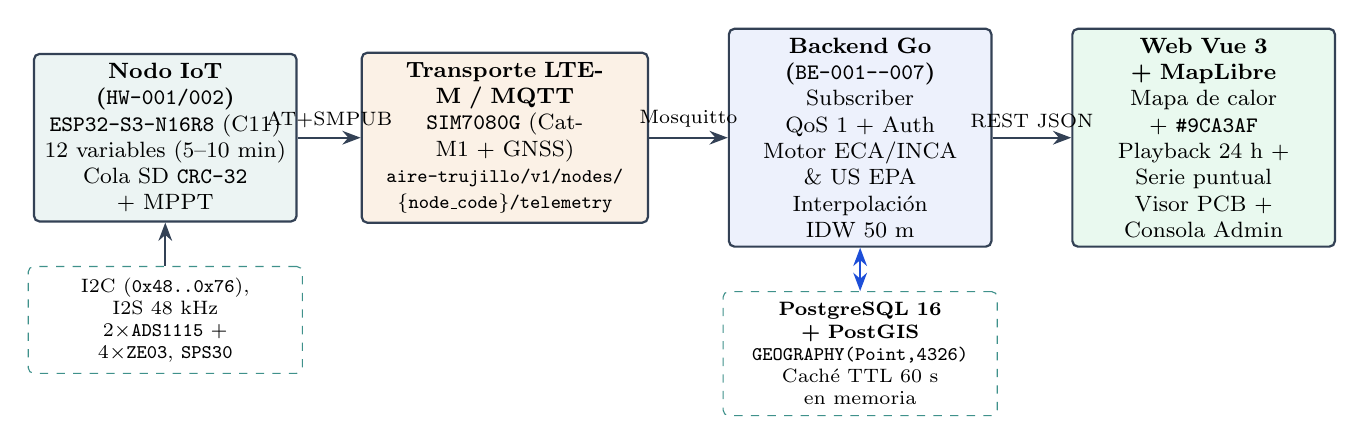
\begin{tikzpicture}[
    node distance=0.6cm and 0.9cm,
    box/.style={rectangle, draw=aireSlate, thick, rounded corners=2pt, minimum height=1.25cm, text width=3.1cm, align=center, font=\footnotesize},
    sub/.style={rectangle, draw=aireTeal!80, dashed, rounded corners=2pt, inner sep=4pt, font=\scriptsize},
    arr/.style={->, >=Stealth, thick, draw=aireSlate},
    darr/.style={<->, >=Stealth, thick, draw=aireBlue}
]
\node[box, fill=aireTeal!8] (hw) {\textbf{Nodo IoT (\texttt{HW-001/002})}\\
\texttt{ESP32-S3-N16R8} (C11)\\
12 variables ($5\text{--}10\text{ min}$)\\
Cola SD \texttt{CRC-32} + MPPT};

\node[box, fill=aireAmber!10, right=0.8cm of hw, text width=3.4cm] (broker) {\textbf{Transporte LTE-M / MQTT}\\
\texttt{SIM7080G} (Cat-M1 + GNSS)\\
{\scriptsize\texttt{aire-trujillo/v1/nodes/}}\\
{\scriptsize\texttt{\{node\_code\}/telemetry}}};

\node[box, fill=aireBlue!8, right=1.0cm of broker] (be) {\textbf{Backend Go (\texttt{BE-001--007})}\\
Subscriber QoS~1 + Auth\\
Motor ECA/INCA \& US~EPA\\
Interpolación IDW $50\text{ m}$};

\node[box, fill=aireGreen!10, right=1.0cm of be] (fe) {\textbf{Web Vue~3 + MapLibre}\\
Mapa de calor + \texttt{\#9CA3AF}\\
Playback $24\text{ h}$ + Serie puntual\\
Visor PCB + Consola Admin};

\node[sub, below=0.55cm of hw, text width=3.2cm, align=center] (sens) {I2C (\texttt{0x48..0x76}), I2S $48\text{ kHz}$\\2$\times$\texttt{ADS1115} + 4$\times$\texttt{ZE03}, \texttt{SPS30}};
\node[sub, below=0.55cm of be, text width=3.2cm, align=center] (db) {\textbf{PostgreSQL~16 + PostGIS}\\ \texttt{GEOGRAPHY(Point,4326)}\\ Caché TTL $60\text{ s}$ en memoria};

\draw[arr] (sens) -- (hw);
\draw[arr] (hw) -- node[above, font=\scriptsize]{AT+SMPUB} (broker);
\draw[arr] (broker) -- node[above, font=\scriptsize]{Mosquitto} (be);
\draw[darr] (be) -- (db);
\draw[arr] (be) -- node[above, font=\scriptsize]{REST JSON} (fe);
\end{tikzpicture}
\caption{Arquitectura integral \emph{end-to-end} de \textbf{aire-trujillo} y acoplamiento estricto bajo el contrato de telemetría Zero-Drift.}
\label{fig:sys_arch}
\end{figure*}

\subsection{Subsistema Energético Solar MPPT y Seccionamiento de Rieles}

El nodo opera autónomamente con celda solar ($5\text{--}18\text{ V}$ en \texttt{J4}) y batería Li-Ion 1S ($3.7\text{ V}$ en \texttt{J5}). El controlador MPPT \texttt{CN3791} (\texttt{U3}, inductor \texttt{L1} $22\ \mu\text{H}$ y resistencia \emph{shunt} \texttt{R18} $0.12\ \Omega\ 1\text{ W}$ para $I_{\mathrm{chg,max}} = 1.0\text{ A}$) fija la tensión de seguimiento del punto de máxima potencia mediante el divisor resistivo \texttt{R10} ($100\text{ k}\Omega$) y \texttt{R11} ($16.5\text{ k}\Omega$)~\cite{consonance2018cn3791}:
\begin{equation}
V_{\mathrm{MPPT}} = 1.205\left(1 + \frac{R_{10}}{R_{11}}\right) = 1.205\left(1 + \frac{100}{16.5}\right) \approx 8.51\text{ V}
\label{eq:mppt}
\end{equation}

Una etapa de selección automática tipo \emph{ORing} basada en MOSFET canal-P \texttt{AO3401A} (\texttt{Q1}, \texttt{Q2}) y diodos Schottky \texttt{SS34} (\texttt{D2}--\texttt{D5}) arbitra la entrada solar, la batería y el puerto USB-C (\texttt{J1}, protegido frente a ESD por \texttt{USBLC6-2SC6} \texttt{U2}) hacia el bus principal \texttt{VSYS}, desacoplado localmente por un banco de baja ESR que incluye \texttt{C32} ($100\ \mu\text{F}$) para amortiguar picos transitorios de transmisión LTE-M de hasta $2\text{ A}$ en \texttt{U8}~\cite{simcom2021sim7080g}. A partir de \texttt{VSYS}, el regulador síncrono Buck \texttt{TLV62569} (\texttt{U4}) genera el riel continuo \texttt{3V3\_SYS} ($3.318\text{ V}$) para el microcontrolador, y el elevador Boost \texttt{TPS61023} (\texttt{U5}, habilitado por \texttt{GPIO21}) produce \texttt{5V\_BOOST} ($4.992\text{ V}$) únicamente durante las ventanas de muestreo~\cite{ti2020power}. Ambos buses periféricos quedan aislados en reposo mediante interruptores de carga \texttt{TPS22919} (\texttt{U7} para \texttt{3V3\_SENS} en \texttt{GPIO48} y \texttt{U6} para \texttt{5V\_SENS} en \texttt{GPIO47}), eliminando corrientes de fuga de sensores, micrófono y tarjeta MicroSD durante el sueño profundo. Adicionalmente, dos canales de \texttt{ADC1} (\texttt{GPIO1} con divisor $\times 2.0$ y \texttt{GPIO2} con $\times 11.0$) junto con las líneas de colector abierto \texttt{CHG\_STAT} (\texttt{GPIO39}) y \texttt{CHG\_DONE} (\texttt{GPIO40}) monitorizan en tiempo real el estado de carga y batería.

\subsection{Instrumentación Multiparamétrica, Frontera Analógica y RF}

La arquitectura sensorial consolida $12$ variables en tres buses del \texttt{ESP32-S3-WROOM-1-N16R8}~\cite{espressif2024esp32s3}, resumidos en la Tabla~\ref{tab:sensor_map}. El bus $\text{I}^2\text{C}$ principal (\texttt{GPIO8/9}, $100\text{ kHz}$ con \emph{pull-ups} externos de $4.7\text{ k}\Omega$ a \texttt{3V3\_SENS}) integra: \texttt{Bosch BME280} (\texttt{0x76})~\cite{bosch2022bme280}, \texttt{Sensirion SCD41} (\texttt{0x62}, fotoacústico NDIR con compensación barométrica)~\cite{sensirion2021scd41}, \texttt{Sensirion SGP40} (\texttt{0x59})~\cite{sensirion2020sgp40}, \texttt{Sensirion SPS30} (\texttt{0x69} sobre \texttt{5V\_SENS} vía \texttt{J9})~\cite{sensirion2020sps30} y dos convertidores ADC delta-sigma de $16\text{ bits}$ \texttt{TI ADS1115} (\texttt{0x48} y \texttt{0x49})~\cite{ti2018ads1115}.

Los cuatro módulos electroquímicos \texttt{Winsen ZE03} ($\text{CO}$, $\text{NO}_2$, $\text{SO}_2$, $\text{H}_2\text{S}$ conectados en \texttt{J10}--\texttt{J13}) proporcionan tanto la salida principal de concentración (\texttt{VO}) como su canal auxiliar libre (\texttt{CORR}) para cancelación de deriva~\cite{winsen2019ze03}. Cada uno de los 8 canales analógicos atraviesa un filtro paso bajo $RC$ de primer orden (\texttt{R45}--\texttt{R52} de $1\text{ k}\Omega$ y \texttt{C54}--\texttt{C61} de $100\text{ nF}$, $f_c = (2\pi R C)^{-1} \approx 1.59\text{ kHz}$) seguido por un doble diodo de sujeción Schottky \texttt{BAT54S} (\texttt{D7}--\texttt{D14}) hacia \texttt{3V3\_SENS} y \texttt{GND}, protegiendo las entradas de \texttt{U14/U15} frente a sobrevoltajes durante la conmutación de $5\text{ V}$. En paralelo, el micrófono MEMS \texttt{ICS-43434} (\texttt{MK1}) se conecta por $\text{I}^2\text{S}$ puro de $24\text{ bits}$ (\texttt{GPIO4/5/6})~\cite{invensense2016ics43434}, mientras la tarjeta MicroSD (\texttt{J2}) usa el bus SPI (\texttt{GPIO10}--\texttt{GPIO14}) y el módem \texttt{SIM7080G} (\texttt{U8}) enlaza por UART (\texttt{GPIO17/18}, \texttt{DTR}, \texttt{STATUS}) mediante el traductor lógico bidireccional $3.3\text{ V} \leftrightarrow 1.8\text{ V}$ \texttt{SN74AVC4T245PW} (\texttt{U9}) y etapas \texttt{BSS138} (\texttt{Q3}/\texttt{Q4})~\cite{simcom2021sim7080g}.

\begin{table}[!t]
\centering
\caption{Asignación de hardware de los 12 parámetros canónicos}
\label{tab:sensor_map}
\footnotesize
\setlength{\tabcolsep}{3.2pt}
\resizebox{\columnwidth}{!}{%
\begin{tabular}{llccc}
\toprule
\textbf{Clave JSON} & \textbf{Sensor / Interfaz} & \textbf{Bus / Dir.} & \textbf{Riel} & \textbf{Rango} \\
\midrule
\texttt{pm25}, \texttt{pm10} & Sensirion SPS30 (\texttt{J9}) & I2C \texttt{0x69} & \texttt{5V\_SENS} & 0--1000 $\mu\text{g/m}^3$ \\
\texttt{co} & ZE03-CO (\texttt{J10}) + U14 & \texttt{0x48} AIN0/1 & \texttt{5V/3V3} & 0--100 $\text{mg/m}^3$ \\
\texttt{no2} & ZE03-NO2 (\texttt{J11}) + U14 & \texttt{0x48} AIN2/3 & \texttt{5V/3V3} & 0--2000 $\mu\text{g/m}^3$ \\
\texttt{so2} & ZE03-SO2 (\texttt{J12}) + U15 & \texttt{0x49} AIN0/1 & \texttt{5V/3V3} & 0--2000 $\mu\text{g/m}^3$ \\
\texttt{h2s} & ZE03-H2S (\texttt{J13}) + U15 & \texttt{0x49} AIN2/3 & \texttt{5V/3V3} & 0--2000 $\mu\text{g/m}^3$ \\
\texttt{co2} & Sensirion SCD41 (\texttt{U12}) & I2C \texttt{0x62} & \texttt{3V3\_SENS} & 400--10000 ppm \\
\texttt{voc\_index} & Sensirion SGP40 (\texttt{U13}) & I2C \texttt{0x59} & \texttt{3V3\_SENS} & 1--500 idx \\
\texttt{noise\_dba} & ICS-43434 (\texttt{MK1}) & I2S $48\text{ kHz}$ & \texttt{3V3\_SENS} & 20--130 dBA \\
\texttt{temperature\_c} & Bosch BME280 (\texttt{U11}) & I2C \texttt{0x76} & \texttt{3V3\_SENS} & $-10\text{--}60\,^\circ\text{C}$ \\
\texttt{humidity\_pct} & Bosch BME280 (\texttt{U11}) & I2C \texttt{0x76} & \texttt{3V3\_SENS} & 0--100 \% \\
\texttt{pressure\_hpa} & Bosch BME280 (\texttt{U11}) & I2C \texttt{0x76} & \texttt{3V3\_SENS} & 800--1100 hPa \\
\bottomrule
\end{tabular}%
}
\end{table}

\subsection{Diseño Físico Multicapa para Entorno Marino (4 Capas ENIG)}

La PCB (\path{hardware/pcb/aire-trujillo.kicad_pcb}, $150.0\text{ mm} \times 105.0\text{ mm}$, esquinas $R=3.0\text{ mm}$ y cuatro anclajes M3 \texttt{H1}--\texttt{H4} para encapsulado IP66 con membrana hidrofóbica ePTFE) emplea el apilado de cuatro capas \texttt{JLC04161H-7628} (espesor $1.60\text{ mm}$, $\varepsilon_r = 4.6$):
\begin{itemize}
    \item \textbf{Capas \texttt{F.Cu} y \texttt{B.Cu} ($35\ \mu\text{m}$ / $1\text{ oz}$):} Enrutamiento ortogonal, par diferencial USB de $90\ \Omega$ (\texttt{GPIO19/20}), líneas RF \emph{Coplanar Waveguide with Ground} (CPWG) de $50\ \Omega$ ($0.30\text{ mm}$ sobre prepreg $0.2104\text{ mm}$) entre \texttt{U8} y los conectores coaxiales \texttt{U.FL} LTE (\texttt{J7}) y GNSS (\texttt{J8}) con valla de vías GND.
    \item \textbf{Capa \texttt{In1.Cu} ($17.5\ \mu\text{m}$):} Plano sólido ininterrumpido de \texttt{GND} como retorno de baja inductancia, con exclusión estricta de cobre bajo la antena impresa de \texttt{U1} ($[10.5,59.5]\times[0.0,7.5]\text{ mm}$) y puerto acústico inferior de \texttt{MK1}.
    \item \textbf{Capa \texttt{In2.Cu} ($17.5\ \mu\text{m}$):} Distribución poligonal de potencia (\texttt{VSYS}, \texttt{VBAT}, \texttt{3V3\_SYS}, \texttt{3V3\_SENS}, \texttt{5V\_BOOST}, \texttt{5V\_SENS}).
\end{itemize}

Para mitigar el autocalentamiento por radiación del regulador, el cargador \texttt{CN3791} y el módem \texttt{SIM7080G}, la península derecha que aloja a \texttt{U11} (\texttt{BME280}), \texttt{U12} (\texttt{SCD41}), \texttt{U13} (\texttt{SGP40}) y \texttt{MK1} queda separada mecánicamente por una ranura fresada de aislamiento térmico (\texttt{Edge.Cuts}, $1.2\text{ mm} \times 18.0\text{ mm}$). Finalmente, cajas de exclusión en \texttt{User.Comments} (\texttt{NO COAT ZONE}) delimitan las zonas libres de recubrimiento conformado sobre sensores de gas/presión/acústica y conectores de servicio. La Fig.~\ref{fig:pcb_renders} exhibe cuatro vistas raytrazadas de la placa fabricable, mientras la Fig.~\ref{fig:schematic_top} muestra la hoja jerárquica raíz del esquemático en KiCad~9.

\begin{figure*}[!t]
\centering
\subfloat[Vista 3D en perspectiva frontal: MCU \texttt{U1}, módem \texttt{U8} y península sensorial derecha.]{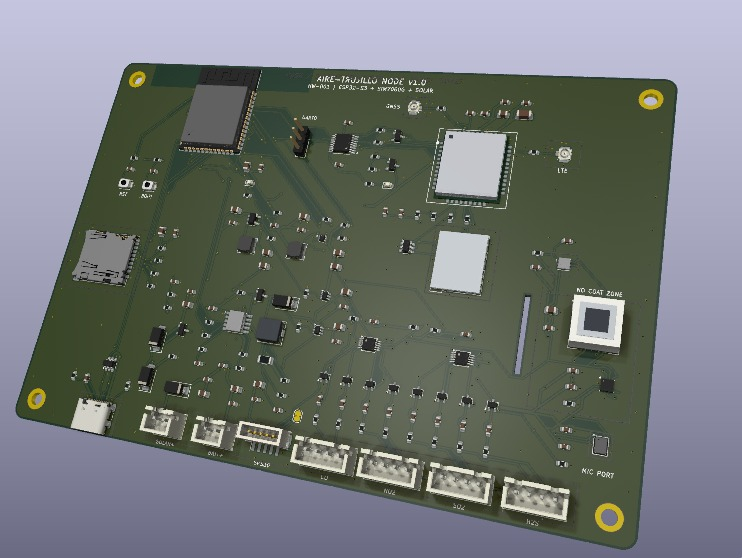
\includegraphics[width=0.485\textwidth]{figures/image.png}\label{fig:pcb_persp1}}
\hfill
\subfloat[Vista 3D isométrica de detalle: conector SIM \texttt{J6}, ranura térmica fresada y regletas \texttt{ZE03}.]{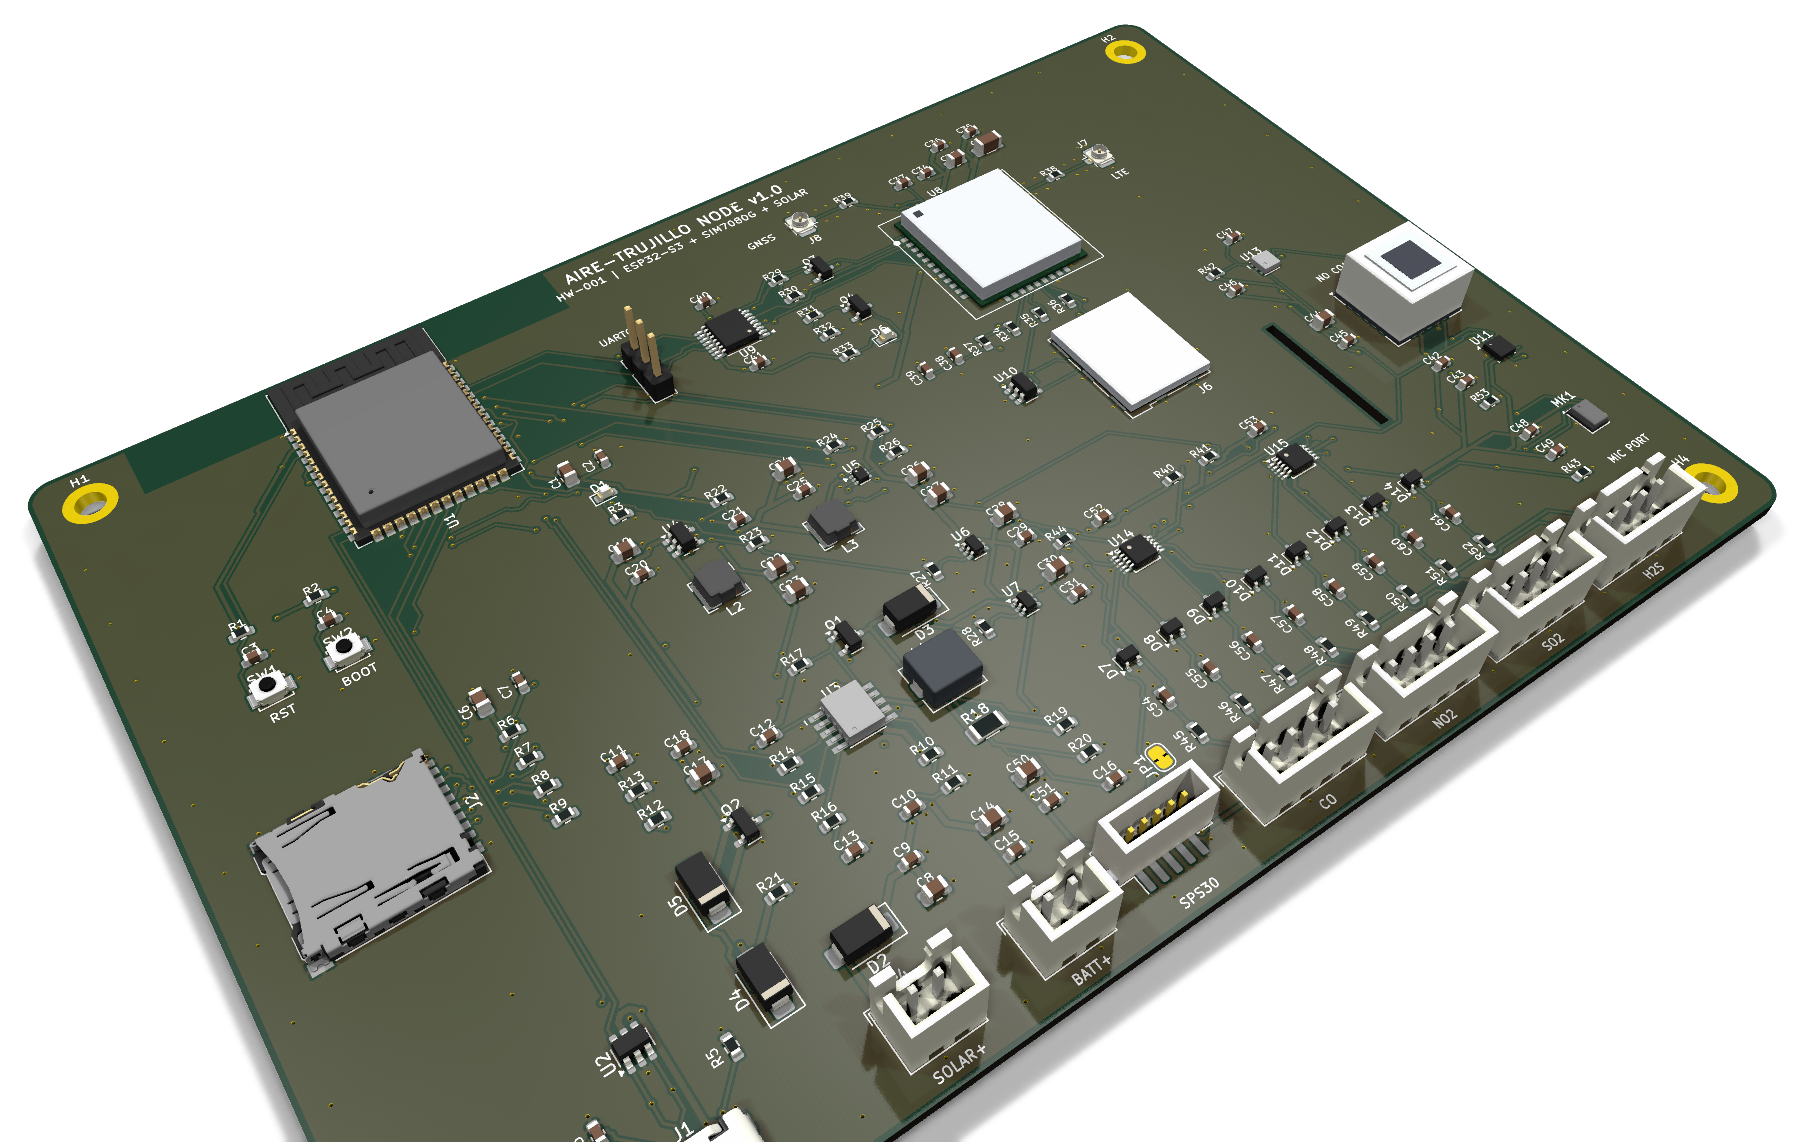
\includegraphics[width=0.485\textwidth]{figures/aire-trujillo-iso-detail.png}\label{fig:pcb_persp2}}\\[4pt]
\subfloat[Vista ortogonal superior (\texttt{F.Cu}): distribución por zonas RF, potencia y sensores.]{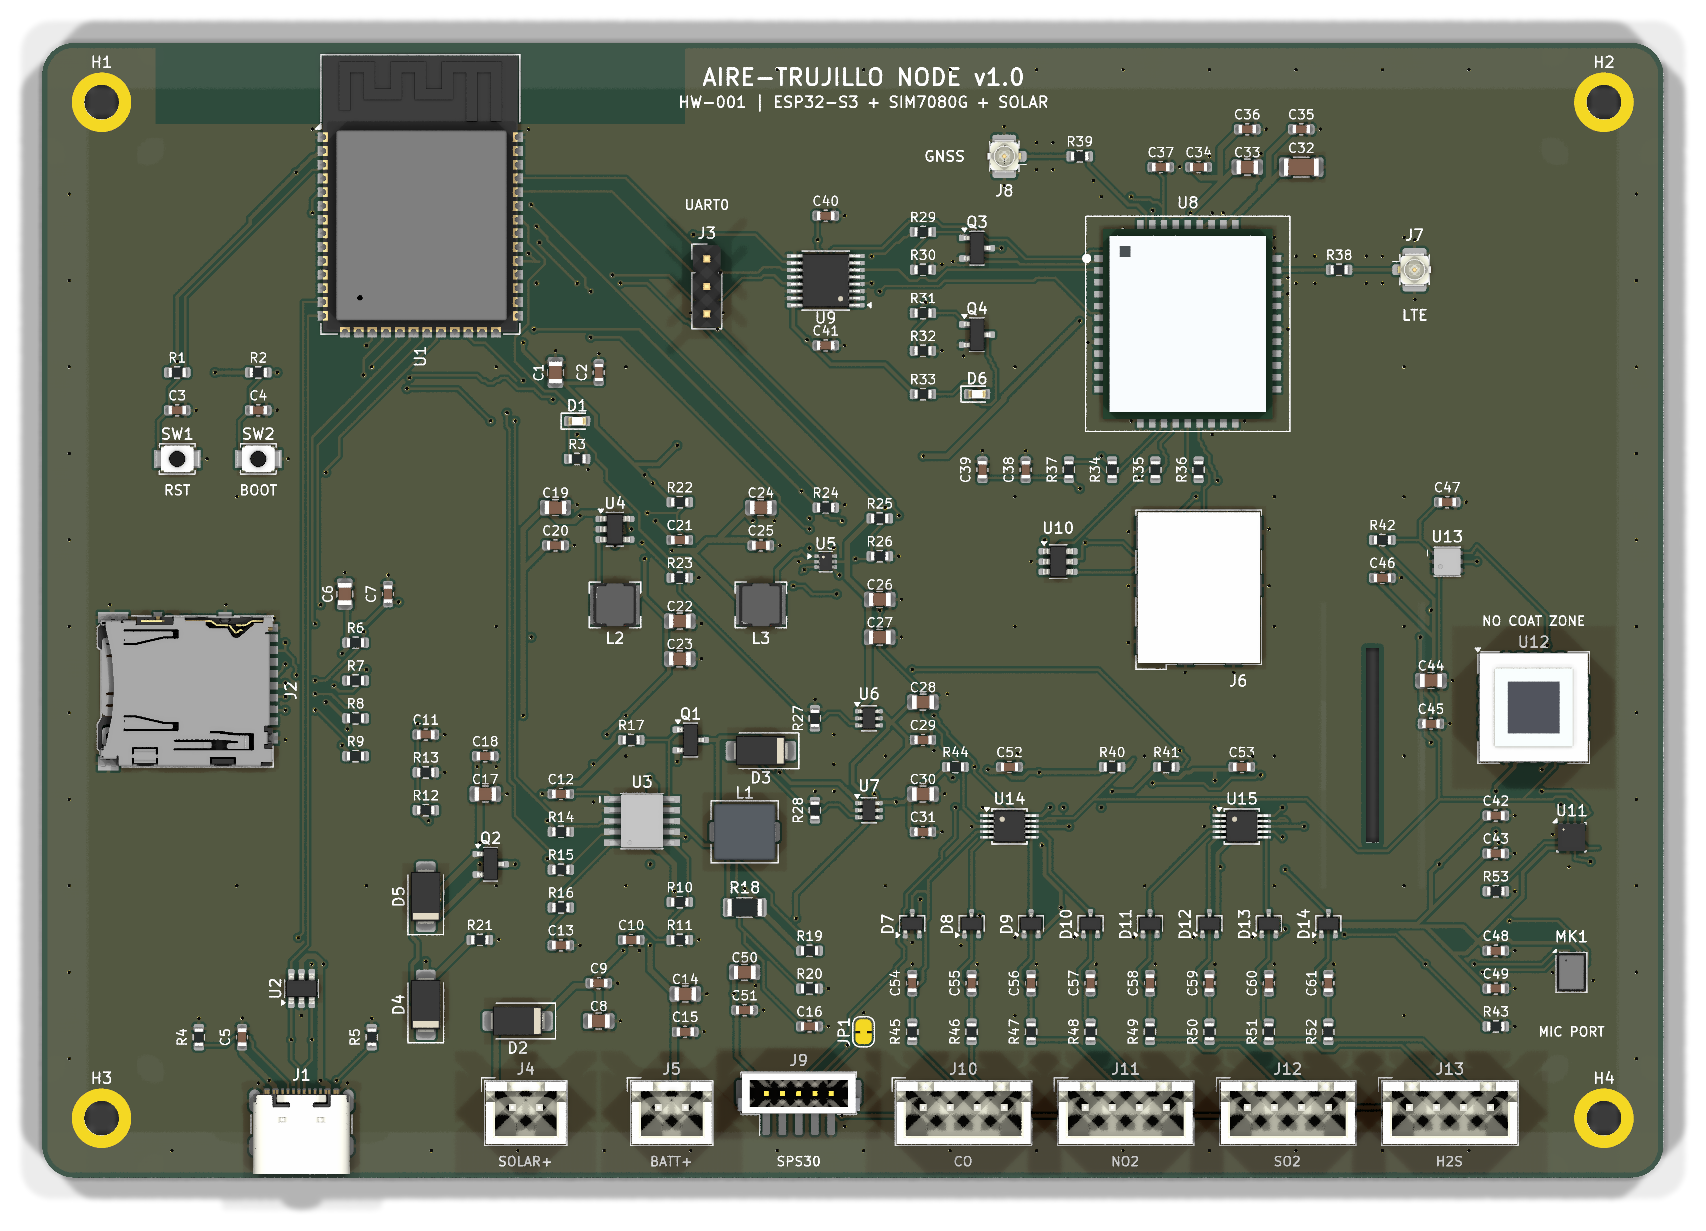
\includegraphics[width=0.485\textwidth]{figures/aire-trujillo-top-crop.png}\label{fig:pcb_top}}
\hfill
\subfloat[Vista ortogonal inferior (\texttt{B.Cu}): plano coplanar GND, vallas de vías RF y ranura térmica.]{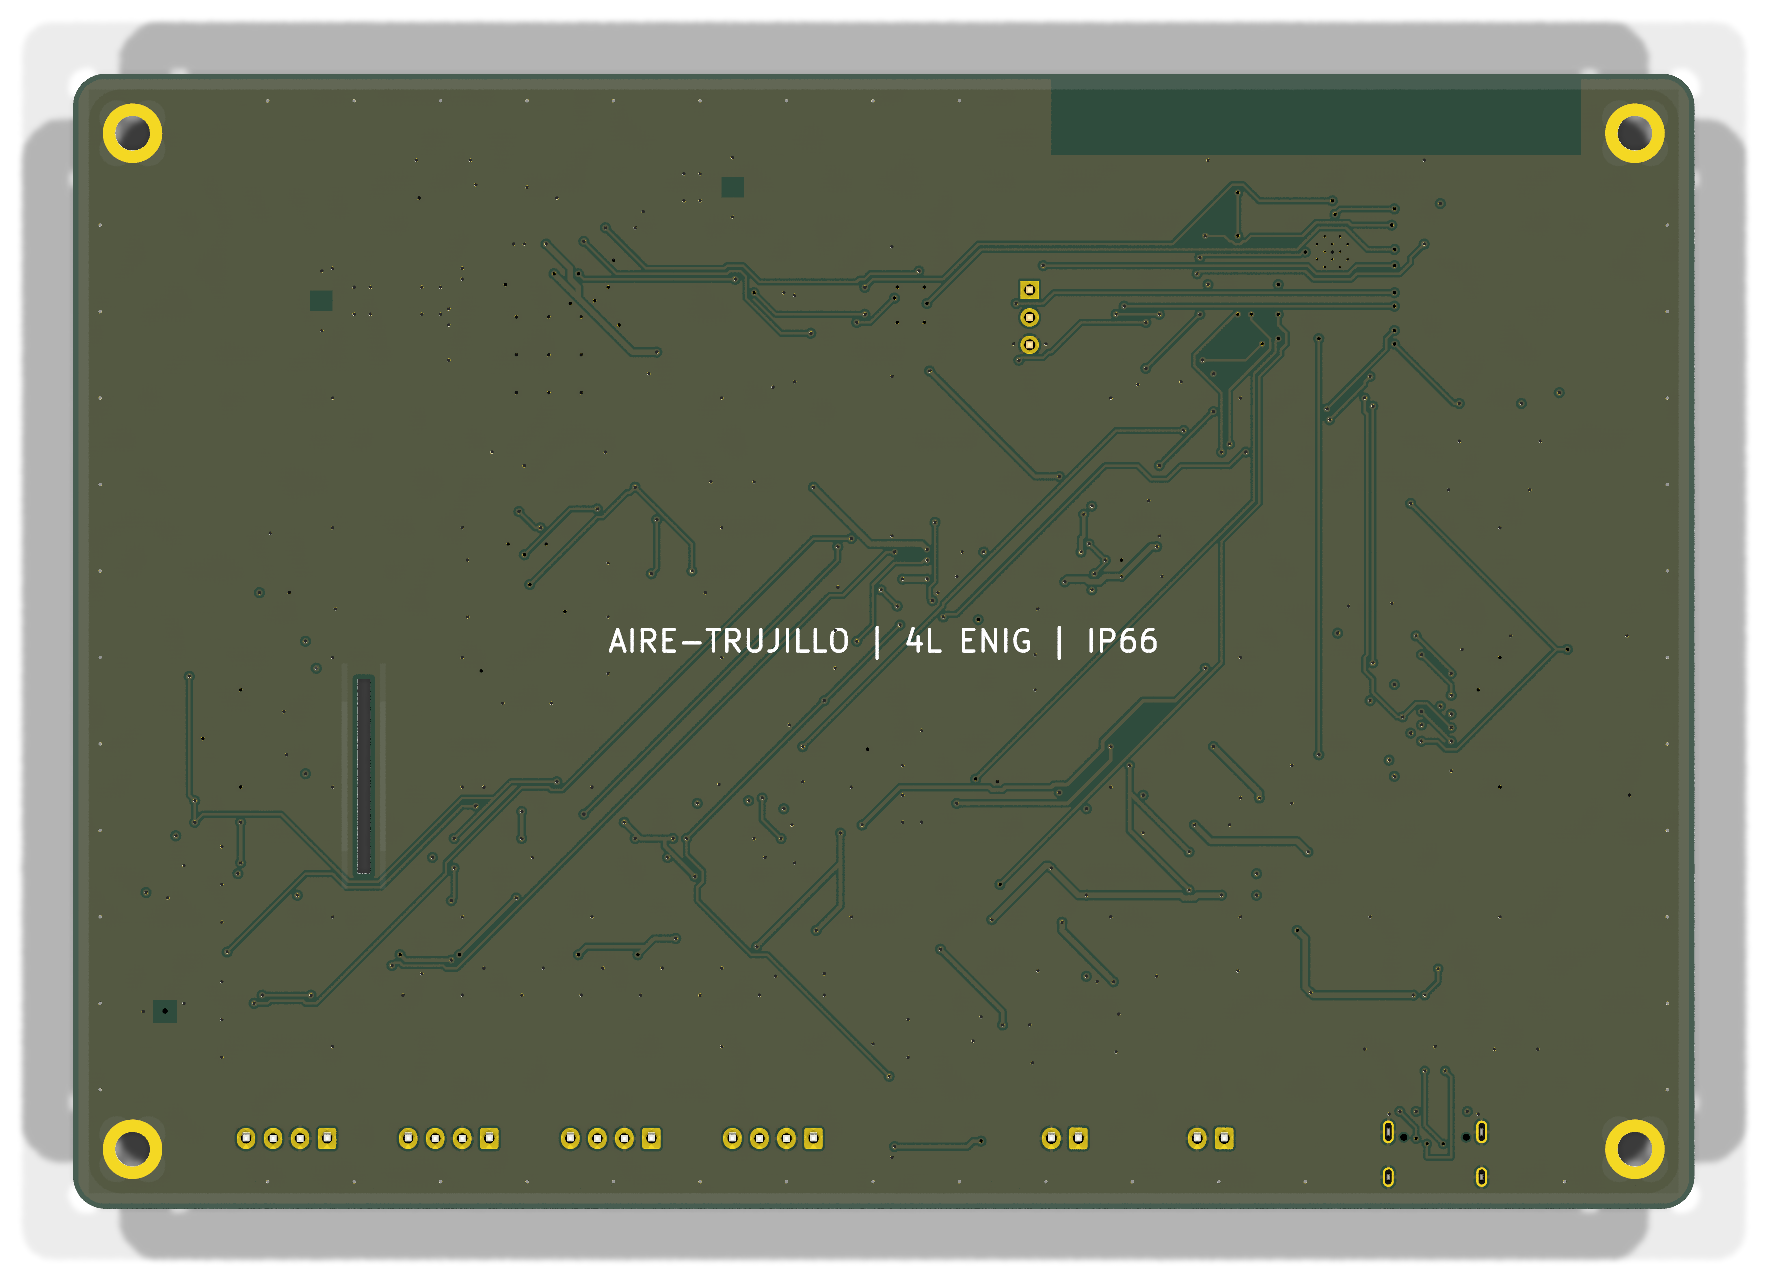
\includegraphics[width=0.485\textwidth]{figures/aire-trujillo-bottom-crop.png}\label{fig:pcb_bot}}
\caption{Renders 3D fotorrealistas de la PCB definitiva de 4 capas ENIG ($150.0\text{ mm} \times 105.0\text{ mm}$, \texttt{aire-trujillo.kicad\_pcb}) generados con el paquete de manufactura en KiCad~9.}
\label{fig:pcb_renders}
\end{figure*}

\begin{figure*}[!t]
\centering
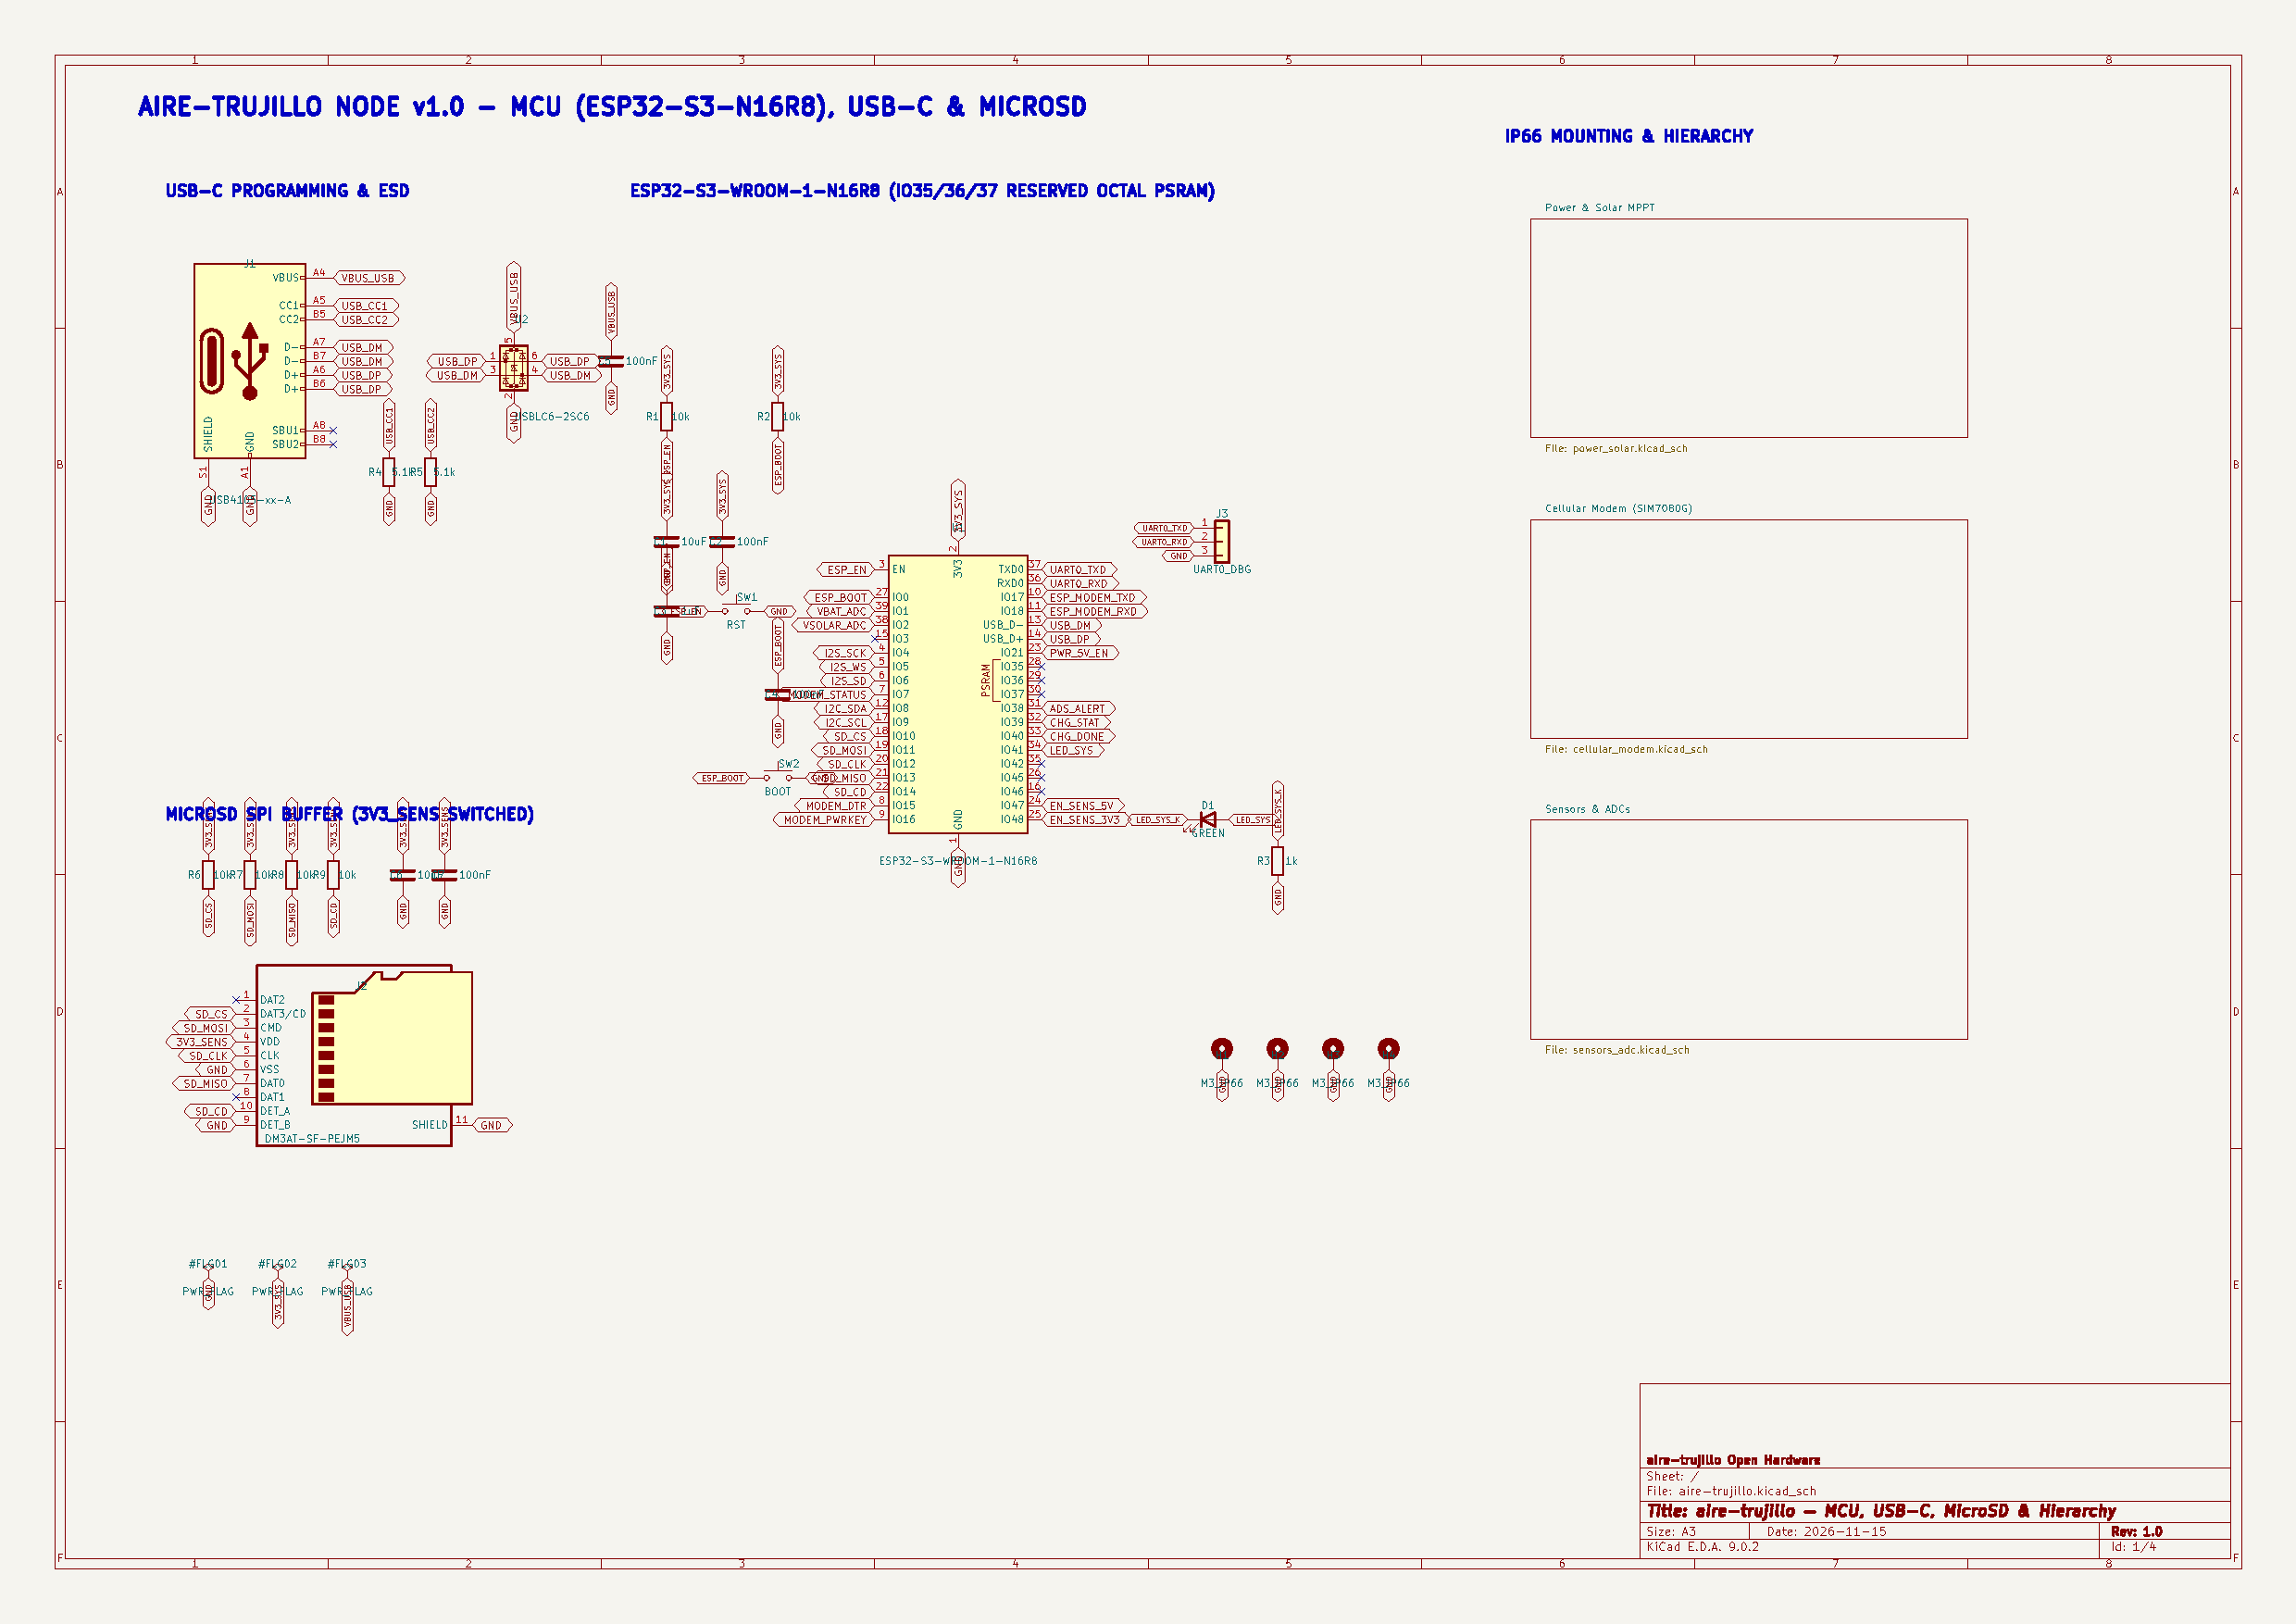
\includegraphics[page=1,width=0.96\textwidth]{figures/aire-trujillo-schematic.pdf}
\caption{Hoja raíz del esquemático jerárquico (\texttt{aire-trujillo.kicad\_sch}) ilustrando el módulo \texttt{ESP32-S3-WROOM-1-N16R8}, las sub-hojas (\texttt{power\_solar}, \texttt{cellular\_modem}, \texttt{sensors\_adc}), interfaz USB-C y socket MicroSD.}
\label{fig:schematic_top}
\end{figure*}

\section{Arquitectura de Firmware Embebido y Procesamiento Digital (\texttt{HW-002})}

\subsection{Decisión C11 + ESP-IDF v5.x y Desacoplamiento Portable}

El firmware del nodo está implementado en \textbf{C11 sobre ESP-IDF v5.x (FreeRTOS)} en lugar de lenguaje ensamblador directo. Esta elección responde a la complejidad de los subsistemas requeridos por \texttt{ESP32-S3-WROOM-1}: pilas \texttt{I2C} maestro, \texttt{I2S DMA} a $48\text{ kHz}$, almacenamiento \texttt{SDSPI + VFS FATFS}, calibración polinomial eFuse de \texttt{ADC1} (\texttt{adc\_cali}), gestión de \texttt{light-sleep}/\texttt{deep-sleep} con retención física de pads (\texttt{gpio\_hold\_en}) y parser UART AT. Para maximizar la verificabilidad previa al despliegue, toda la lógica matemática y de protocolos reside en el componente independiente \texttt{aire\_core}, compilable de manera idéntica en servidor Linux mediante \texttt{gcc -std=c11} y en el compilador cruzado Xtensa LX7.

\subsection{Calibración Electroquímica, Sensores Digitales y Compensación Cruzada}

En sensores digitales Sensirion (\texttt{SCD41}, \texttt{SGP40}, \texttt{SPS30}), toda palabra de $16\text{ bits}$ es validada por firmware mediante CRC-8 con polinomio $0x31$ e inicialización $0x\text{FF}$ antes de aceptarla~\cite{sensirion2020sps30,sensirion2021scd41}. Las tramas de temperatura, humedad y presión barométrica del \texttt{BME280} (\texttt{0xF7..0xFE}) se compensan empleando las constantes de fábrica almacenadas en los registros \texttt{0x88..0xA1} y \texttt{0xE1..0xE7}~\cite{bosch2022bme280}, alimentando inmediatamente la compensación barométrica del \texttt{SCD41} (\texttt{0xE000}) y los \emph{ticks} de compensación termohigrométrica del \texttt{SGP40} (\texttt{0x260F}). El índice VOC preserva una línea base adaptativa exponencial (\emph{EWMA}, $\alpha = 0.02$) en memoria \texttt{RTC\_DATA\_ATTR} no volátil durante el sueño profundo.

Para los cuatro sensores electroquímicos \texttt{Winsen ZE03}, configurados los dos \texttt{ADS1115} en rango $\pm 4.096\text{ V}$ ($0.125\text{ mV/LSB}$, promedio de $4$ muestras por canal a $128\text{ SPS}$), el firmware aplica un rechazo previo de canales flotantes o en cortocircuito fuera de ventana ($[150, 3150]\text{ mV}$). Posteriormente calcula la deriva compartida de línea base mediante la señal auxiliar \texttt{CORR} y la sensibilidad térmica relativa respecto a $T_{\mathrm{ref}} = 25\,^\circ\text{C}$~\cite{mead2013electrochemical,winsen2019ze03}:
\begin{equation}
V_{\mathrm{net}} = \max\!\left(0,\; V_{\mathrm{VO}} - g_c\,(V_{\mathrm{CORR}} - V_{\mathrm{corr},0}) - V_{\mathrm{zero}}\right)
\label{eq:ze03_net}
\end{equation}
\begin{equation}
C_{\mathrm{ppm}} = \frac{V_{\mathrm{net}}}{V_{\mathrm{span}}}\frac{C_{\mathrm{FS}}}{1 + k_T(T_{\mathrm{amb}} - 25.0)},\;
C_{\mathrm{mg/m}^3} = \frac{M C_{\mathrm{ppm}}}{24.45}
\label{eq:ze03_conc}
\end{equation}
donde $M \in \{28.01, 46.01, 64.07, 34.08\}\text{ g/mol}$ representa las masas molares de $\text{CO}$, $\text{NO}_2$, $\text{SO}_2$ y $\text{H}_2\text{S}$, escalando en un factor $10^3$ para las especies expresadas en $\mu\text{g/m}^3$. Si el pin \texttt{CORR} no está poblado en un módulo de reemplazo ($<150\text{ mV}$), \texttt{sensors\_hal.c} degrada de forma segura a compensación térmica pura sin introducir desplazamiento espurio.

\subsection{Cadena DSP Acústica IEC~61672-1 a \texorpdfstring{$48\text{ kHz}$}{48 kHz}}

El flujo $\text{I}^2\text{S}$ mono de $24\text{ bits}$ del micrófono \texttt{ICS-43434} a $f_s = 48\text{ kHz}$ descarta los primeros $4\,096$ muestros ($\approx 85\text{ ms}$) durante el establecimiento del filtro de decimación interno, y captura luego $72\,000$ muestras ($1.5\text{ s}$) procesadas bloque a bloque con: (a) un filtro bloqueador DC de primer orden ($\alpha = 0.995$), (b) una cascada de tres secciones biquad de segundo orden diseñadas por transformación bilineal exacta del filtro analógico de ponderación~A según IEC~61672-1~\cite{iec61672} (normalizada a $0.015\text{ dB}$ en $1\text{ kHz}$ y $-19.75\text{ dB}$ en $100\text{ Hz}$, Fig.~\ref{fig:biquad_freq}), y (c) cálculo de nivel equivalente $\mathrm{dBA}$ referido al punto nominal del MEMS ($94.0\text{ dB SPL} \equiv -26.0\text{ dBFS}$ en onda senoidal)~\cite{invensense2016ics43434}:
\begin{equation}
L_{A} = 20\log_{10}\!\left(\frac{\mathrm{RMS}(y)}{1/\sqrt{2}}\right) + 120.0 + \Delta_{\mathrm{cal}}
\label{eq:dba}
\end{equation}

\begin{figure}[!t]
\centering
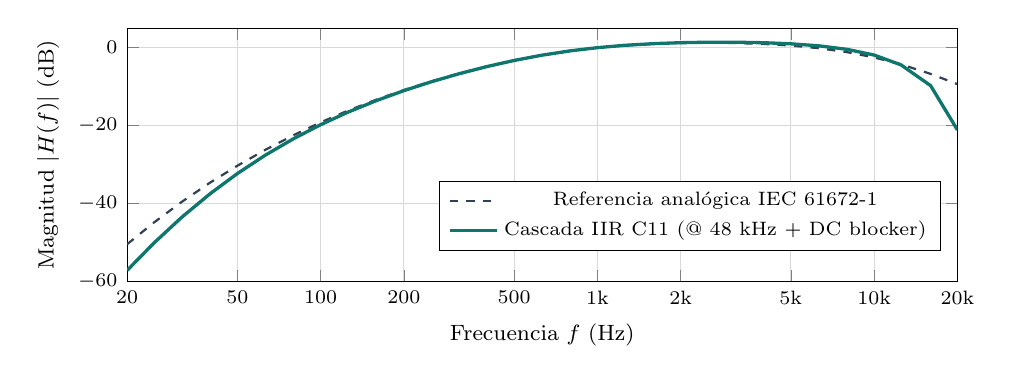
\begin{tikzpicture}
\begin{semilogxaxis}[
    width=\columnwidth,
    height=4.8cm,
    grid=both,
    minor grid style={gray!15},
    major grid style={gray!30},
    xmin=20, xmax=20000,
    ymin=-60, ymax=5,
    xlabel={Frecuencia $f$ (Hz)},
    ylabel={Magnitud $|H(f)|$ (dB)},
    legend style={at={(0.98,0.12)},anchor=south east,font=\scriptsize},
    xtick={20,50,100,200,500,1000,2000,5000,10000,20000},
    xticklabels={20,50,100,200,500,1k,2k,5k,10k,20k},
    tick label style={font=\scriptsize},
    label style={font=\footnotesize}
]
\addplot[color=aireSlate, dashed, thick] coordinates {
(20,-50.395) (25,-44.821) (31.5,-39.529) (40,-34.539) (50,-30.275)
(63,-26.223) (80,-22.398) (100,-19.145) (125,-16.190) (160,-13.244)
(200,-10.847) (250,-8.675) (315,-6.644) (400,-4.774) (500,-3.248)
(630,-1.909) (800,-0.795) (1000,0.000) (1250,0.576) (1600,0.993)
(2000,1.202) (2500,1.271) (3150,1.201) (4000,0.963) (5000,0.554)
(6300,-0.116) (8000,-1.147) (10000,-2.492) (12500,-4.254) (16000,-6.706) (20000,-9.347)
};
\addlegendentry{Referencia analógica IEC~61672-1}

\addplot[color=aireTeal, very thick] coordinates {
(20,-57.090) (25,-50.072) (31.5,-43.476) (40,-37.371) (50,-32.286)
(63,-27.595) (80,-23.301) (100,-19.747) (125,-16.587) (160,-13.494)
(200,-11.011) (250,-8.782) (315,-6.713) (400,-4.816) (500,-3.273)
(630,-1.919) (800,-0.792) (1000,0.015) (1250,0.608) (1600,1.049)
(2000,1.291) (2500,1.408) (3150,1.411) (4000,1.280) (5000,1.004)
(6300,0.491) (8000,-0.425) (10000,-1.881) (12500,-4.388) (16000,-9.719) (20000,-21.073)
};
\addlegendentry{Cascada IIR C11 (@ 48 kHz + DC blocker)}
\end{semilogxaxis}
\end{tikzpicture}
\caption{Respuesta en frecuencia exacta de la cascada digital biquad + bloqueador DC implementada en \texttt{aire\_calibration.c} a $48\text{ kHz}$ frente a la curva analógica estándar IEC~61672-1~\cite{iec61672}.}
\label{fig:biquad_freq}
\end{figure}

\subsection{Secuencia de Potencia, Reloj UTC y Store-and-Forward}

La gestión energética (\texttt{app\_main.c} y \texttt{aire\_power\_evaluate\_budget}) sigue una máquina de estados estrictamente secuenciada para impedir superposiciones entre la corriente del ventilador \texttt{SPS30}/boost de $5\text{ V}$ y la ráfaga de transmisión RF de \texttt{SIM7080G} (Fig.~\ref{fig:power_cycle}):
\begin{enumerate}
    \item \emph{Protección de batería:} Si $V_{\mathrm{BAT}} < 3250\text{ mV}$, se inhiben los sensores de $5\text{ V}$ y LTE-M, extendiendo el intervalo de sueño profundo $4\times$. Entre $3250$ y $3500\text{ mV}$ sin luz solar ($V_{\mathrm{SOL}} < 4500\text{ mV}$), el ciclo se duplica ($2\times$).
    \item \emph{Adquisición y light-sleep:} Se energiza \texttt{3V3\_SENS} antes de iniciar I2C y se activa \texttt{5V\_SENS}; mientras \texttt{SPS30} y \texttt{ZE03} completan el calentamiento ($\sim 25\text{ s}$), se leen \texttt{BME280}, \texttt{SCD41}, \texttt{SGP40} e \texttt{ICS-43434}, tras lo cual el MCU entra en \texttt{esp\_light\_sleep\_start()} reteniendo sus GPIOs. Concluida la lectura de particulado y los 8 canales \texttt{ADS1115}, \textbf{se apaga por completo el boost de $5\text{ V}$} antes de activar la radio celular.
    \item \emph{Sincronización horaria UTC híbrida:} Tras registrar LTE-M (\texttt{AT+CNMP=38}, \texttt{AT+CMNB=1}), \texttt{aire\_modem\_sync\_utc} consulta primero el fijado GNSS (\texttt{+CGNSINF}); si el equipo opera sin vista directa al cielo, utiliza NITZ (\texttt{AT+CCLK?}) aplicando conversión aritmética civil exacta para transformar la hora local peruana (\texttt{-20} cuartos de hora = $\text{UTC}-5$) a formato UTC ISO-8601 (\texttt{Z}), manejando cambios de medianoche y años bisiestos.
    \item \emph{Cola persistente en MicroSD:} Cada muestra válida es anexada en \texttt{/sdcard/queue.log} como línea tabular \texttt{|CRC32|topic\textbackslash tjson\textbackslash n}. Un archivo auxiliar \texttt{/sdcard/queue.idx} actualizado mediante archivo temporal y \texttt{rename()} atómico rastrea la cabeza FIFO: ante cortes de energía a mitad de escritura, las líneas truncadas son descartadas automáticamente por validación \texttt{CRC-32}, drenando hasta $32$ tramas acumuladas vía \texttt{AT+SMPUB} QoS~1 en cuanto se restablece el enlace celular.
\end{enumerate}

\begin{figure}[!t]
\centering
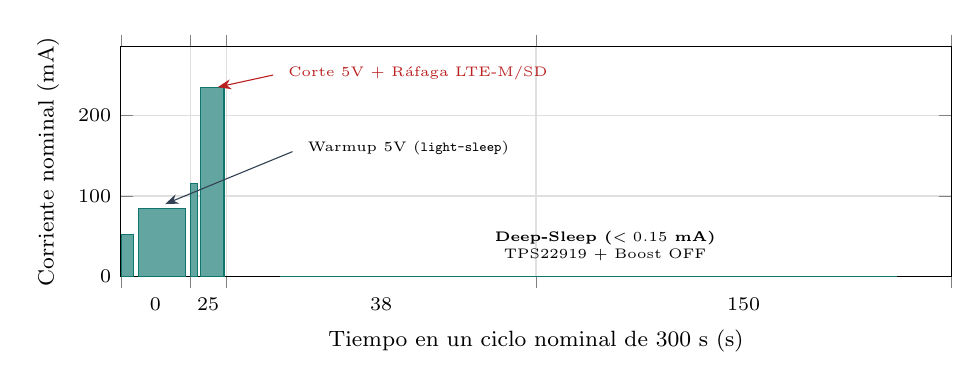
\begin{tikzpicture}
\begin{axis}[
    width=\columnwidth,
    height=4.5cm,
    ybar interval=0.85,
    xmin=0, xmax=300,
    ymin=0, ymax=285,
    xlabel={Tiempo en un ciclo nominal de 300 s (s)},
    ylabel={Corriente nominal (mA)},
    grid=major,
    major grid style={gray!25},
    xtick={0,25,38,150,300},
    xticklabels={0,25,38,150,300},
    tick label style={font=\scriptsize},
    label style={font=\footnotesize}
]
\addplot[fill=aireTeal!65, draw=aireTeal] coordinates {
(0, 52)     % Boot + ADC + BME280 + SCD41 + SGP40
(5, 85)     % Light-sleep + SPS30 fan + 4x ZE03 warmup
(25, 115)   % Read SPS30 + 2x ADS1115 + SD append
(28, 235)   % Cutoff 5V_SENS + SIM7080G LTE-M / MQTT QoS1 burst
(38, 0.15)  % Deep sleep (load switches OFF via gpio_hold_en)
(300, 0.15)
};
\draw[->, >=Stealth, aireSlate] (axis cs:62,155) -- (axis cs:16,90);
\node[font=\tiny, align=left, anchor=west] at (axis cs:64,160) {Warmup 5V (\texttt{light-sleep})};
\draw[->, >=Stealth, aireRed!85!black] (axis cs:55,250) -- (axis cs:35,235);
\node[font=\tiny, align=left, anchor=west, text=aireRed!85!black] at (axis cs:57,252) {Corte 5V + Ráfaga LTE-M/SD};
\node[font=\tiny, align=center] at (axis cs:175,38) {\textbf{Deep-Sleep ($<0.15\text{ mA}$)}\\TPS22919 + Boost OFF};
\end{axis}
\end{tikzpicture}
\caption{Perfil nominal de consumo eléctrico por etapas durante un ciclo estándar de $300\text{ s}$ (estimado por hojas de datos~\cite{espressif2024esp32s3,simcom2021sim7080g,sensirion2020sps30,ti2020power} con exclusión mutua entre riel de $5\text{ V}$ y ráfaga celular).}
\label{fig:power_cycle}
\end{figure}

\section{Motor Geoespacial Backend e Interpolación IDW con Decaimiento de Confianza (\texttt{BE-001}--\texttt{BE-007})}

\subsection{Contrato Zero-Drift y Esquema PostGIS}

Para garantizar coherencia sin derivas entre hardware, backend y visualización, tanto el serializador \texttt{aire\_telemetry.c} como el suscriptor MQTT (\texttt{backend/internal/mqtt/subscriber.go}) y el repositorio de PostgreSQL~16 (\texttt{PostGIS 3.4}) implementan idénticas reglas de validación:
\begin{enumerate}
    \item Las 12 métricas comparten exactamente las mismas claves \texttt{snake\_case} y límites plausibles (Tabla~\ref{tab:sensor_map}). Todo campo omitido por desconexión puntual o falla de CRC llega como \texttt{null} en SQL y \texttt{*float64 = nil} en Go, prohibiéndose el reemplazo por cero.
    \item La localización geográfica se almacena en coordenadas geodésicas \texttt{GEOGRAPHY(Point, 4326)} con índice espacial \texttt{GIST}, mientras la tabla \texttt{telemetry\_readings} indexa \texttt{(node\_id, recorded\_at DESC)} bajo clave única compuesta para idempotencia frente a retransmisiones QoS~1 del firmware.
    \item La autenticación del panel administrativo utiliza verificación en memoria constante de frase secreta salada con hash criptográfico (\texttt{BE-002}), emitiendo sesión HTTP-only sin exponer pistas en respuestas no autorizadas.
\end{enumerate}

\subsection{Formulación Espacial IDW con Degradado Explícito Hacia Gris}

Dado un conjunto de nodos activos $k \in \mathcal{N}_t$ con lectura válida dentro de la ventana temporal $[t - 15\text{ min},\, t]$, el motor (\texttt{backend/internal/spatial/idw.go}) genera una grilla dinámica de paso cuadrado $\Delta = 50\text{ m}$ centrada sobre la envolvente de los nodos con margen $R_{\max} = 600\text{ m}$ (protegida por un tope de $250\,000$ celdas para ejecución segura en presupuestos de memoria reducidos). La distancia geodésica $d_k(\mathbf{x})$ entre el centro de cada celda $\mathbf{x}=(\phi,\lambda)$ y el nodo $k$ se evalúa mediante la fórmula de Haversine ($R_{\oplus}=6\,371\,000\text{ m}$).

El campo interpolado $\hat{v}(\mathbf{x})$ mediante ponderación inversa de la distancia~\cite{shepard1968idw} con exponente $p=2$ se evalúa únicamente sobre el subconjunto activo local $\mathcal{K}(\mathbf{x}) = \{k \in \mathcal{N}_t : d_k(\mathbf{x}) \le R_{\max}\}$:
\begin{equation}
\hat{v}(\mathbf{x}) =
\begin{cases}
v_{k^*}, & \text{si } \exists\, k^* : d_{k^*}(\mathbf{x}) < 1\text{ m} \\
\dfrac{\sum_{k \in \mathcal{K}(\mathbf{x})} d_k(\mathbf{x})^{-2}\, v_k}{\sum_{k \in \mathcal{K}(\mathbf{x})} d_k(\mathbf{x})^{-2}}, & \text{si } \mathcal{K}(\mathbf{x}) \neq \varnothing \\
\texttt{null}, & \text{si } \mathcal{K}(\mathbf{x}) = \varnothing
\end{cases}
\label{eq:idw}
\end{equation}

Sea $d_{\min}(\mathbf{x}) = \min_{k \in \mathcal{N}_t} d_k(\mathbf{x})$ la distancia al sensor más próximo. El parámetro de confianza espacial $C(\mathbf{x}) \in [0, 1]$ modela la degradación progresiva de representatividad entre $R_{\mathrm{fade}} = 400\text{ m}$ y $R_{\max} = 600\text{ m}$:
\begin{equation}
C(\mathbf{x}) = \operatorname{clip}_{[0,1]}\!\left(1 - \frac{d_{\min}(\mathbf{x}) - R_{\mathrm{fade}}}{R_{\max} - R_{\mathrm{fade}}}\right)
\label{eq:confidence}
\end{equation}
A partir de $C(\mathbf{x})$, cada celda con cobertura mezcla linealmente en espacio sRGB el color categórico base $\mathbf{c}_{\mathrm{base}}$ con el gris neutro de incertidumbre $\mathbf{c}_{\mathrm{gris}} = (156, 163, 175)$ (\texttt{\#9CA3AF}), tal como grafica la Fig.~\ref{fig:idw_confidence}:
\begin{equation}
\mathbf{c}_{\mathrm{final}}(\mathbf{x}) = \operatorname{round}\!\big(C(\mathbf{x})\,\mathbf{c}_{\mathrm{base}} + (1 - C(\mathbf{x}))\,\mathbf{c}_{\mathrm{gris}}\big)
\label{eq:rgb_blend}
\end{equation}
Fuera de $R_{\max}$, las consultas devuelven explícitamente \texttt{has\_data = false}, \texttt{value = null}, \texttt{confidence = 0.0} y etiqueta \texttt{"No hay datos"}, suprimiendo cualquier ilusión visual en zonas carentes de instrumentación.

\begin{figure}[!t]
\centering
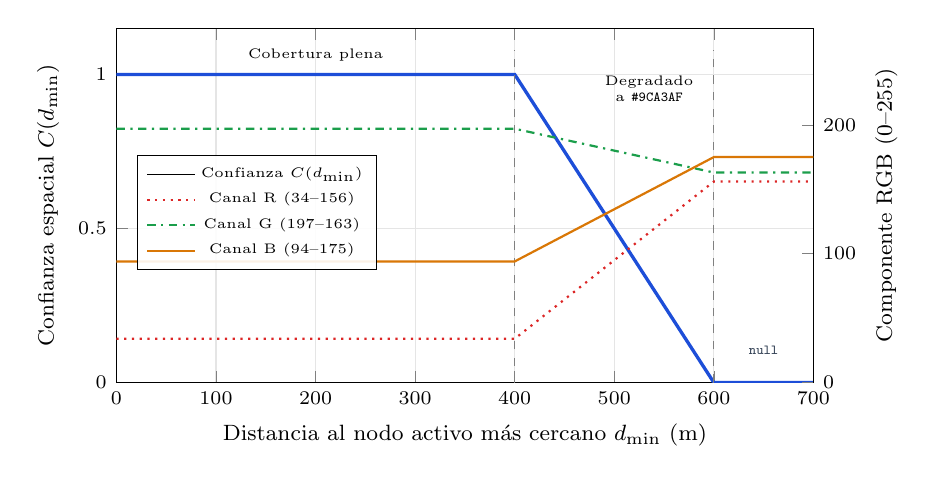
\begin{tikzpicture}
\begin{axis}[
    width=0.73\columnwidth,
    height=4.5cm,
    scale only axis,
    xmin=0, xmax=700,
    ymin=0, ymax=1.15,
    axis y line*=left,
    xlabel={Distancia al nodo activo más cercano $d_{\min}$ (m)},
    ylabel={Confianza espacial $C(d_{\min})$},
    grid=major,
    major grid style={gray!20},
    tick label style={font=\scriptsize},
    label style={font=\footnotesize}
]
\addplot[color=aireBlue, very thick] coordinates {
(0, 1.0) (400, 1.0) (600, 0.0) (700, 0.0)
};
\label{plot:conf}

\draw[dashed, gray] (axis cs:400,0) -- (axis cs:400,1.08);
\draw[dashed, gray] (axis cs:600,0) -- (axis cs:600,1.08);
\node[font=\tiny, anchor=south] at (axis cs:200,1.01) {Cobertura plena};
\node[font=\tiny, align=center, anchor=south] at (axis cs:535,0.88) {Degradado\\a \texttt{\#9CA3AF}};
\node[font=\tiny, anchor=south, text=aireSlate] at (axis cs:650,0.06) {\texttt{null}};
\end{axis}

\begin{axis}[
    width=0.73\columnwidth,
    height=4.5cm,
    scale only axis,
    xmin=0, xmax=700,
    ymin=0, ymax=275,
    axis y line*=right,
    axis x line=none,
    ylabel={Componente RGB (0--255)},
    legend style={at={(0.03,0.48)},anchor=west,font=\tiny,fill=white,fill opacity=0.9,text opacity=1},
    tick label style={font=\scriptsize},
    label style={font=\footnotesize}
]
\addlegendimage{/pgfplots/refstyle=plot:conf}\addlegendentry{Confianza $C(d_{\min})$}
\addplot[color=aireRed, thick, dotted] coordinates {(0,34) (400,34) (600,156) (700,156)};
\addlegendentry{Canal R (34--156)}
\addplot[color=aireGreen!80!black, thick, dashdotted] coordinates {(0,197) (400,197) (600,163) (700,163)};
\addlegendentry{Canal G (197--163)}
\addplot[color=aireAmber, thick] coordinates {(0,94) (400,94) (600,175) (700,175)};
\addlegendentry{Canal B (94--175)}
\end{axis}
\end{tikzpicture}
\caption{Decaimiento espacial de confianza $C(d_{\min})$ entre $R_{\mathrm{fade}}=400\text{ m}$ y $R_{\max}=600\text{ m}$ junto con la transición lineal de canales RGB desde categoría \emph{Buena} (\texttt{\#22C55E}) hacia gris neutro (\texttt{\#9CA3AF}).}
\label{fig:idw_confidence}
\end{figure}

\section{Plataforma Cartográfica Interactiva y Gemelo de Simulación (\texttt{FE-001}--\texttt{FE-007})}

La capa de presentación está construida en \texttt{Vue~3}, \texttt{TypeScript} y \texttt{MapLibre GL}, estructurada en tres vistas especializadas:
\begin{itemize}
    \item \textbf{Landing interactiva y Visor PCB (\texttt{HomeView.vue}, \texttt{PcbExplorer.vue}):} Explica la arquitectura solar/IoT para Trujillo y Huanchaco e integra un inspector de módulos que permite seleccionar bloques clave de la placa (\texttt{ESP32-S3}, \texttt{SIM7080G}, \texttt{SPS30}, \texttt{ZE03}, \texttt{SCD41}, \texttt{SGP40}, \texttt{BME280}, \texttt{ICS-43434}, \texttt{CN3791} y MicroSD) mostrando su función y variables asociadas.
    \item \textbf{Mapa geoespacial vivo (\texttt{MapView.vue}, \texttt{IdwCoverageProbe.vue}):} Renderiza las celdas de $50\text{ m}$ provenientes de \texttt{GET /api/v1/map/heatmap} con conmutación inmediata entre el estándar principal \textbf{ECA/INCA}~\cite{minam2016inca}, \textbf{US~EPA~AQI}~\cite{usepa2024aqi} y las $12$ variables individuales. Al hacer clic en cualquier coordenada del dominio, consulta \texttt{GET /api/v1/map/point} obteniendo el valor puntual interpolado, la confianza y la evolución histórica de $24\text{ h}$, complementado por un control de \emph{playback} temporal y una caché en memoria de $60\text{ s}$ que se invalida automáticamente al ingresar telemetría MQTT.
    \item \textbf{Consola administrativa discreta (\texttt{EditView.vue}):} Accesible sin pistas públicas mediante verificación de frase secreta (\texttt{POST /api/v1/access/verify}), habilita el alta georreferenciada de nodos y la inyección en lote (\texttt{/admin/nodes/\{id\}/readings/batch}) de series de $24\text{ h}$ cada $5\text{ min}$ (ej. tráfico hora punta en el Centro Histórico o episodio costero en Huanchaco) para validar el comportamiento del motor IDW y el front-end previo al montaje en calle.
\end{itemize}

\section{Evaluación Experimental, Verificación de Calidad y Discusión}

Siguiendo los criterios trazables de control de calidad establecidos para el proyecto (\texttt{03-quality-and-testing.md}), la evaluación se ejecutó sobre cuatro frentes independientes sin emplear datos inventados.

\subsection{Verificación Eléctrica, Manufactura PCB y Pruebas de Firmware}

En KiCad~9, la auditoría eléctrica (\texttt{kicad-cli sch erc --severity-all}) sobre las 4 hojas del esquemático jerárquico ($171$ símbolos, $66$ líneas únicas de lista de materiales \texttt{BOM}) y la verificación física (\texttt{kicad-cli pcb drc --severity-all --schematic-parity}) sobre la placa terminada arrojaron \textbf{cero errores y cero advertencias} con $95/95$ redes enrutadas ($0$ ítems sin conectar y paridad esquemático-PCB exacta), generando el paquete completo de fabricación JLCPCB ENIG (Gerbers X2, taladros PTH/NPTH, archivo \texttt{POS} de centroides Top/Bottom y modelo sólido STEP).

El núcleo portable \texttt{C11} del firmware (\texttt{aire\_core}) fue compilado bajo reglas estrictas (\texttt{-std=c11 -Wall -Wextra -Werror -Wpedantic -Wconversion -Wshadow}) y verificado con \texttt{ctest}, superando \textbf{100\% de las pruebas} (\texttt{test\_firmware\_core}) con cero advertencias:
\begin{itemize}
    \item \emph{Sensores y calibración:} Validación CRC-8 con vector oficial Sensirion (\texttt{0xBEEF} $\to$ \texttt{0x92}), vector de compensación oficial Bosch \texttt{BME280} ($25.08\,^\circ\text{C}$, $1006.53\text{ hPa}$ dentro de $\pm 0.02\,^\circ\text{C}$ / $\pm 0.05\text{ hPa}$), decodificación IEEE-754 big-endian de $60\text{ bytes}$ \texttt{SPS30} con rechazo de corrupción de $1\text{ bit}$, y sustracción de deriva compartida ($+30\text{ mV}$) entre canales \texttt{VO} y \texttt{CORR} del \texttt{Winsen ZE03-CO} manteniendo error menor a $0.01\text{ mg/m}^3$.
    \item \emph{DSP acústico:} Ante tono puro de $1\text{ kHz}$ a $-26\text{ dBFS}$ ($f_s=48\text{ kHz}$), la cascada computó $94.0 \pm 0.35\text{ dBA}$ incluso en presencia de polarización DC ($+0.08$ FS), y verificó la atenuación normativa a $100\text{ Hz}$ ($-19.17\text{ dB}$ dentro de $\pm 0.7\text{ dB}$).
    \item \emph{Resiliencia store-and-forward y AT:} Se comprobó la recuperación automática tras inyectar una trama truncada con CRC corrupto en \texttt{queue.log}, la compactación circular acotada por \texttt{max\_bytes}, la conversión NITZ de cruce de medianoche y año bisiesto (\texttt{"28/02/29,23:30:00-20"} $\to$ \texttt{"2028-03-01T04:30:00Z"}), y la secuencia completa de publicación \texttt{AT+SMPUB} QoS~1.
    \item \emph{Compatibilidad binaria con Go:} Una trama JSON real emitida por el binario compilado en C ($264\text{ bytes}$ de payload sobre tópico de $49\text{ bytes}$) fue validada sin errores mediante \texttt{json.NewDecoder} con \texttt{DisallowUnknownFields()} y parser temporal \texttt{RFC3339}. El chequeo sintáctico de \texttt{app\_main.c}, \texttt{bus\_hal.c} y \texttt{sensors\_hal.c} frente a cabeceras \emph{stub} de ESP-IDF resultó en $0$ errores; queda únicamente pendiente ejecutar \texttt{idf.py build} en una estación con el SDK completo de Espressif instalado y la calibración en cámara de prototipo físico.
\end{itemize}

\subsection{Cobertura del Backend y Escalabilidad Espacial IDW}

La ejecución integral de la suite en Go (\texttt{go test -cover ./...}) reportó la cobertura real de sentencias resumida en la Tabla~\ref{tab:qc_summary}, destacando un $76.6\%$ en el núcleo espacial (\texttt{internal/spatial}), $69.8\%$ en autenticación y $68.8\%$ en simulación. La cobertura de \texttt{internal/store} ($5.4\%$) obedece a la ausencia de instancia PostgreSQL en las pruebas unitarias aisladas.

Para dimensionar la viabilidad del servicio en despliegues de capa gratuita (\emph{free tier}), se cronometró el algoritmo IDW de grilla de $50\text{ m}$ mediante un \emph{harness} nativo en Go (\texttt{go run}) promediado sobre $100$ ejecuciones calientes en cuatro topologías progresivas sobre Trujillo (Tabla~\ref{tab:idw_bench} y Fig.~\ref{fig:idw_perf}). Incluso al escalar de un nodo aislado ($576$ celdas, $0.221\text{ ms}$) a un corredor metropolitano de $16$ estaciones ($4\,928$ celdas sobre $4.2 \times 3.4\text{ km}$), la latencia de cálculo se mantiene en \textbf{6.231 ms} con solo $388.2\text{ KB}$ asignados por invocación y un payload JSON de $567.4\text{ KB}$, que al almacenarse en caché de $60\text{ s}$ resulta fácilmente asumible por instancias de bajos recursos.

\begin{table}[!t]
\centering
\caption{Resumen de evidencias verificadas de hardware, firmware y backend}
\label{tab:qc_summary}
\footnotesize
\resizebox{\columnwidth}{!}{%
\begin{tabular}{lll}
\toprule
\textbf{Módulo / Artefacto} & \textbf{Criterio / Herramienta} & \textbf{Resultado Verificado} \\
\midrule
Esquemático PCB (4 hojas) & \texttt{kicad-cli sch erc} & $0$ errores, $0$ adv. ($171$ símb.) \\
PCB 4L ENIG + Manufactura & \texttt{kicad-cli pcb drc} & $0$ viol., $95/95$ redes, paridad OK \\
Núcleo Firmware \texttt{C11} & \texttt{cmake + ctest} (\texttt{-Werror}) & \textbf{100\% aprobado} ($1/1$ suite, $0$ warn.) \\
Contrato C $\leftrightarrow$ Go & \texttt{DisallowUnknownFields} & Decodificación OK ($264\text{ B}$ JSON) \\
Compilación cruzada MCU & \texttt{idf.py build} (\texttt{esp32s3}) & Pendiente (SDK no instalado) \\
\midrule
Backend \texttt{internal/spatial} & \texttt{go test -cover} & $76.6\%$ cobertura ($7\text{ ms}$) \\
Backend \texttt{internal/auth} & \texttt{go test -cover} & $69.8\%$ cobertura \\
Backend \texttt{internal/simulator} & \texttt{go test -cover} & $68.8\%$ cobertura \\
Backend \texttt{internal/aqi} & \texttt{go test -cover} & $47.8\%$ cobertura \\
Backend \texttt{internal/api} & \texttt{go test -cover} & $46.8\%$ cobertura \\
Backend \texttt{internal/mqtt} & \texttt{go test -cover} & $43.9\%$ cobertura \\
\bottomrule
\end{tabular}%
}
\end{table}

\begin{table}[!t]
\centering
\caption{Desempeño del algoritmo IDW ($50\text{ m}$) sobre cuatro despliegues en Trujillo}
\label{tab:idw_bench}
\footnotesize
\setlength{\tabcolsep}{4pt}
\resizebox{\columnwidth}{!}{%
\begin{tabular}{lcccc}
\toprule
\textbf{Escenario} & \textbf{Grilla / Celdas} & \textbf{Lat. (ms)} & \textbf{JSON (KB)} & \textbf{Alloc (KB)} \\
\midrule
1 nodo ($1.2\times1.2\text{ km}$) & $24\times25$ ($576$) & 0.221 & 66.6 & 51.5 \\
4 nodos ($1.8\times1.8\text{ km}$) & $40\times40$ ($1\,560$) & 0.603 & 181.9 & 128.3 \\
8 nodos ($2.8\times2.4\text{ km}$) & $51\times38$ ($1\,887$) & 1.301 & 217.9 & 157.5 \\
16 nodos ($4.2\times3.4\text{ km}$) & $78\times64$ ($4\,928$) & 6.231 & 567.4 & 388.2 \\
\bottomrule
\end{tabular}%
}
\end{table}

\begin{figure}[!t]
\centering
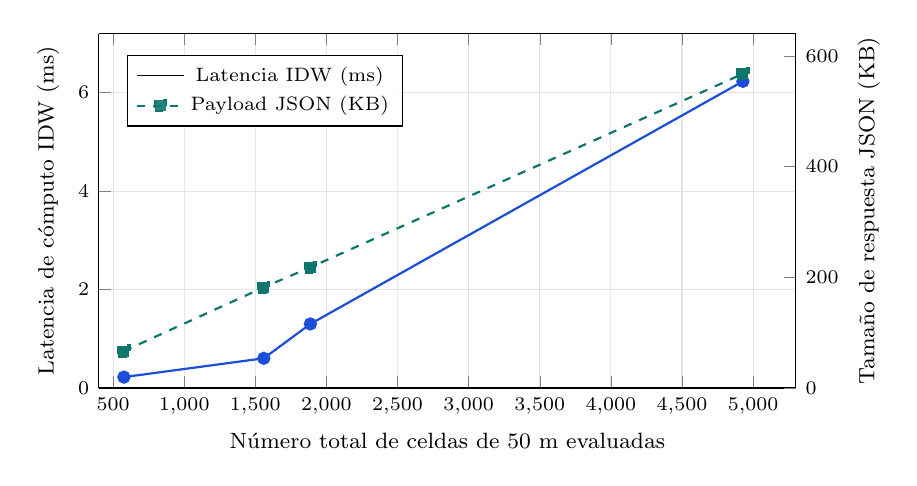
\begin{tikzpicture}
\begin{axis}[
    width=0.73\columnwidth,
    height=4.5cm,
    scale only axis,
    xmin=400, xmax=5300,
    ymin=0, ymax=7.2,
    axis y line*=left,
    xlabel={Número total de celdas de $50\text{ m}$ evaluadas},
    ylabel={Latencia de cómputo IDW (ms)},
    grid=major,
    major grid style={gray!20},
    tick label style={font=\scriptsize},
    label style={font=\footnotesize}
]
\addplot[color=aireBlue, mark=*, thick] coordinates {
(576, 0.221) (1560, 0.603) (1887, 1.301) (4928, 6.231)
};
\label{plot:lat}
\end{axis}

\begin{axis}[
    width=0.73\columnwidth,
    height=4.5cm,
    scale only axis,
    xmin=400, xmax=5300,
    ymin=0, ymax=640,
    axis y line*=right,
    axis x line=none,
    ylabel={Tamaño de respuesta JSON (KB)},
    legend style={at={(0.04,0.94)},anchor=north west,font=\scriptsize,fill=white,fill opacity=0.9,text opacity=1},
    tick label style={font=\scriptsize},
    label style={font=\footnotesize}
]
\addlegendimage{/pgfplots/refstyle=plot:lat}\addlegendentry{Latencia IDW (ms)}
\addplot[color=aireTeal, mark=square*, thick, dashed] coordinates {
(576, 66.6) (1560, 181.9) (1887, 217.9) (4928, 567.4)
};
\addlegendentry{Payload JSON (KB)}
\end{axis}
\end{tikzpicture}
\caption{Escalabilidad empírica de latencia de cómputo y tamaño de respuesta JSON del motor IDW en Go en función del tamaño de grilla evaluada sobre escenarios urbanos en Trujillo.}
\label{fig:idw_perf}
\end{figure}

\section{Conclusiones y Trabajo Futuro}

Se diseñó y verificó integralmente \textbf{aire-trujillo}, articulando hardware solar multiparamétrico IP66 de cuatro capas, firmware resiliente en \texttt{C11} con DSP acústico y cola \texttt{MicroSD} tolerante a fallos, backend espacial en \texttt{Go/PostGIS} y plataforma web interactiva. El aporte central radica en la trazabilidad estricta entre niveles: el contrato Zero-Drift evita sustituir datos faltantes por ceros en toda la cadena, en tanto el decaimiento lineal de confianza entre $400\text{ m}$ y $600\text{ m}$ transparenta los límites físicos de cobertura de la red de sensores sin penalizar el rendimiento computacional ($<6.3\text{ ms}$ para $4\,928$ celdas).

Como trabajo futuro inmediato se contempla: (1) fabricar el primer lote piloto de PCB ENIG y compilar/flashear la imagen definitiva sobre silicio mediante \texttt{idf.py build}; (2) ejecutar campañas de co-localización junto a estaciones de referencia del Ministerio del Ambiente (MINAM) para ajustar regresiones de calibración multivariada específicas de los módulos \texttt{ZE03} bajo humedad costera~\cite{zimmerman2018machinemean}; y (3) desplegar pruebas continuas de autonomía solar y cobertura LTE-M entre el Centro Histórico de Trujillo y el litoral de Huanchaco.

\IEEEtriggeratref{15}
\bibliographystyle{ieeetr}
\bibliography{references}

\end{document}
